\section{THIẾT KẾ PHẦN CỨNG}
\subsection{Tổng quan hệ thống}
\subsubsection{Giới thiệu}
Hệ thống CNN (Convolutional Neural Network) được thiết kế trong tài liệu này tập trung vào việc phân tích ảnh xám và dự đoán chữ số từ 0 đến 9 dưới dạng mã BCD (Binary-Coded Decimal), kết hợp giữa kiến trúc phần cứng tối ưu và thuật toán học sâu. Mô-đun CNN áp dụng ý tưởng thiết kế hệ thống số về mô-đun điều khiển/xử lý dữ liệu, chia toàn bộ mạng nhận dạng thành hai khối chính:
\begin{itemize}
    \item \textbf{Khối điều khiển (máy trạng thái FSM)} Phát lệnh điều khiển dựa trên tín hiệu và trạng thái từ khối xử lý dữ liệu.
    \item  \textbf{Khối xử lý dữ liệu (Datapath)} Nhận lệnh từ khối điều khiển để thực hiện tính toán và phản hồi trạng thái hiện tại.
\end{itemize}

\subsubsection{Sơ đồ thiết kế phần cứng}
\begin{figure}[H]
    \centering
    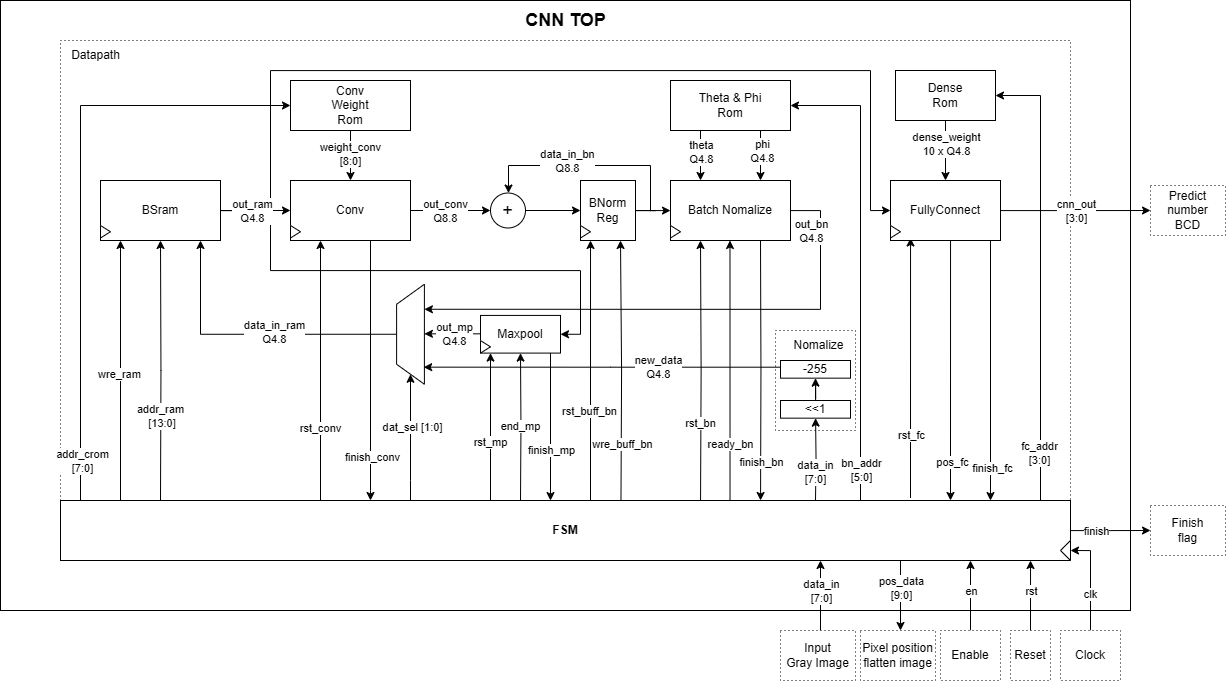
\includegraphics[angle=-90, width=0.75\linewidth]{Images/datapath_cnn.drawio.png}
    \caption{Sơ đồ thiết kế phần cứng khối CNN}
    \label{fig:tkpc}
\end{figure}


\subsubsection{Mục tiêu thiết kế}
\begin{itemize}
    \item \textbf{Xử lý ảnh hiệu quả:} Tiếp nhận đầu vào là điểm ảnh xám 8-bit, kết hợp theo dõi vị trí để tối ưu bộ nhớ.
    \item \textbf{Tối ưu tài nguyên:} Sử dụng định dạng dấu phẩy tĩnh (Q4.8, Q8.8) để cân bằng độ chính xác và chi phí tính toán. Việc sử dụng nhiều các khối chuẩn hóa giúp cho dữ liệu sau khi tính toán giao động từ $[-1; 1]$ do đó chọn địn dạng số có dấu Q4.8 với tầm từ $[-8; 7.99609375]$ lượng tử với độ phân giải $\frac{1}{256}$. Dữ liệu trung gian Q8.8 để dự phòng cho trường hợp ngõ vào của khối Batch Normalize là tổng tích chập nhiều \textit{Window} (Tối đa là 8 \textit{Window} với mô hình của đề tài) với nhau, ngoài ra Q8.8 còn sử dụng trong ruột của khối Fully Connect.
\end{itemize}

\subsubsection{Thông số kỹ thuật chính}

Thiết kế pipeline xử lý ảnh xám đầu vào qua 4 giai đoạn chính: Convolution → Batch Normalization → Max Pooling → Fully Connected.

\begin{itemize}
    \item \textbf{Định dạng dữ liệu:}
    \begin{itemize}
        \item Đầu vào: 8-bit grayscale + 10-bit vị trí (pos\_data[9:0]).
        \item Trung gian: Q4.8/Q8.8 fixed-point.
        \item Đầu ra: 4-bit BCD (cnn\_out[3:0])
    \end{itemize}

    \item \textbf{Bộ nhớ:}
    \begin{itemize}
        \item BRAM 14-bit address (addr\_ram[13:0])
        \item 3 ROM chứa:
        \begin{itemize}
            \item Conv weights (9-bit)
            \item Theta/Phi params (Q4.8) (Đề cập sau)
            \item Dense layer weights (Q4.8)
        \end{itemize}
    \end{itemize}

\end{itemize}

\subsubsection{Đặc Điểm Nổi Bật}
\begin{itemize}
    \item \textbf{Kiến trúc phần cứng rõ ràng:} ách biệt khối xử lý (Convolution, BN, Pooling, FC) và điều khiển (FSM), đồng bộ qua các tín hiệu \textit{finish} và \textit{rst}.
    \item \textbf{Bộ nhớ chuyên biệt:} ROM lưu trọng số tích chập (9-bit) và tham số chuẩn hóa (Q4.8), BRAM lưu dữ liệu trung gian với địa chỉ 14-bit.
    \item \textbf{Đầu ra linh hoạt:} Kết quả dự đoán 4-bit BCD, phù hợp với các hệ thống nhúng hoặc giao tiếp vi điều khiển.
\end{itemize}

\subsection{Khối tích chập (Binary Convolution)}
\subsubsection{Ý Tưởng Thiết Kế}
\begin{itemize}
    \item Thiết kế một bộ tích chập (convolution unit) tối ưu cho xử lý tín hiệu số với:
    \begin{itemize}
        \item Đầu vào dạng fixed-point Q4.8 (12-bit)
        \item Đầu ra dạng Q8.8 (16-bit)
        \item Hỗ trợ kernel 3x3 (9 trọng số)
    \end{itemize}
    \item Kết hợp 2 module chính:
    \begin{itemize}
        \item \textit{SIPO19:} Chuyển đổi serial-to-parallel 1 to 9 cho từng bit dữ liệu
        \item \textit{conv:} Thực hiện phép tích chập bằng cách ghép 12 bộ SIPO19 độc lập và thực hiện phép cộng trừ dựa theo trọng số nhị phân.
    \end{itemize}
    \begin{figure}[H]
        \centering
        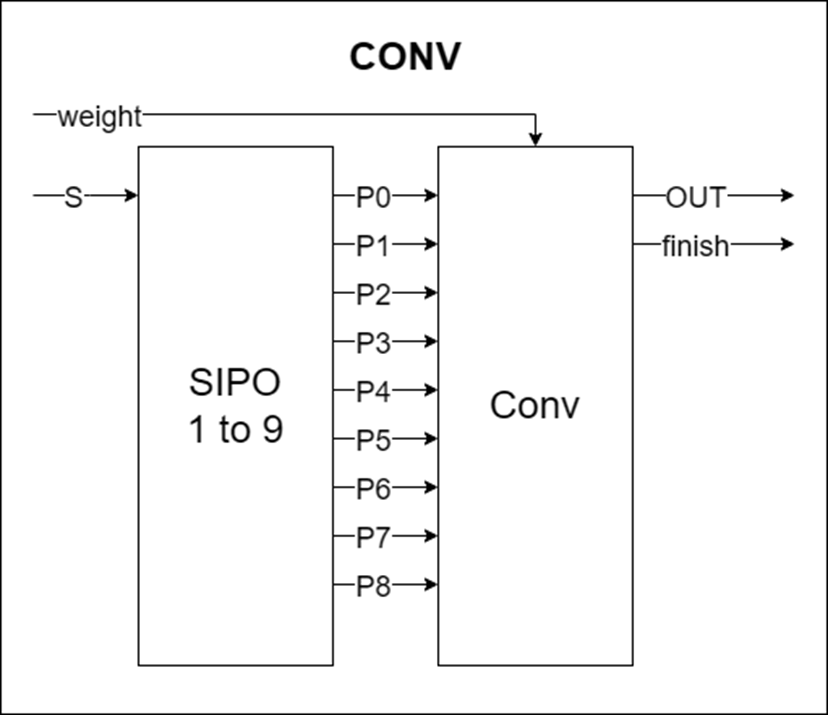
\includegraphics[width=0.75\linewidth]{Images/conv.png}
        \caption{Sơ đồ khối Binary Conv}
        \label{fig:enter-label}
    \end{figure}
    \item Sử dụng counter 4-bit để điều khiển luồng dữ liệu.
    \item Triển khai phép nhân qua thao tác XOR và cộng đơn giản. 
    \begin{verbatim}
        d_w[i] = (n_data[i]^{12{w[i]}})+{11'b0,w[i]}
    \end{verbatim}
\end{itemize}


\subsubsection{Thiết kế khối SIPO19}
\begin{verbatim}
    module SIPO19 (
    input clk, reset, serial_in, shift,
    output reg [8:0] parallel_out
    );
\end{verbatim}
\begin{itemize}
    \item Chức năng: 
    \begin{itemize}
        \item Dịch 9 bit nối tiếp → song song
        \item Giữ kết quả ở \textit{parallel\_out} khi \textit{shift=1}
    \end{itemize}
    \item Đặc điểm thiết kế:
    \begin{itemize}
        \item Thanh ghi 9-bit \textit{shift\_registe}r dịch trái mỗi chu kỳ clock
        \item Reset đồng bộ xóa cả thanh ghi và đầu ra
    \end{itemize}
\end{itemize}

\subsubsection{Thiết kế khối Conv}
\begin{table}[h]
\centering
\caption{Module Binary Convolution Signal Definitions}
\label{tab:signals}
\begin{tabular}{llll}
\toprule
\textbf{Signal Name} & \textbf{Direction} & \textbf{Width} & \textbf{Description} \\
\midrule
clk & Input & 1 & System clock \\
rst & Input & 1 & Active-high reset \\
en\_conv & Input & 1 & Convolution enable \\
data\_in & Input & 12 & Input data (Q4.8 format) \\
w & Input & 9 & Weight vector (0=add, 1=subtract) \\
finish & Output & 1 & Operation completion flag \\
out & Output & 16 & Result (Q8.8 format) \\
\bottomrule
\end{tabular}
\end{table}


\begin{itemize}
    \item Cơ chế hoạt động: 
    \begin{itemize}
        \item Giai đoạn load dữ liệu:
        \begin{itemize}
            \item 12 SIPO19 thu nhận từng bit của \textit{data\_in} khi \textit{sync=1}
            \item Mỗi SIPO19 tạo 9 bản sao song song của 1 bit dữ liệu
        \end{itemize}
        \item Giai đoạn tính toán:
        \begin{itemize}
            \item Tạo 9 phiên bản dữ liệu đã chuẩn hóa (\textit{d\_w[0:8]})
            \item Tính tổng có dấu với sign extension (bit mở rộng dấu)
        \end{itemize}
        \item Giai đoạn hoàn tất conv: Counter đếm đến 10 chu kỳ → báo \textit{finish}
    \end{itemize}
    \item Phép Toán Tích Chập
    \begin{itemize}
        \item Cơ chế nhân nhị phân: Với mỗi trọng số \textit{w[i]}
        \begin{itemize}
            \item Nếu \textit{w[i]=1}: Thực hiện phép đảo bit và cộng 1 (bù 2)
            \item Nếu \textit{w[i]=0}: Giữ nguyên giá trị
        \end{itemize}
        \item Mở rộng dấu 4 bit trước khi tính tổng (từ 12-bit → 16-bit)
    \end{itemize}
\end{itemize}


\subsubsection{Kiểm Thử \& Xác Minh}
\begin{table}[h]
\centering
\caption{Binary Convolution Verification Plan Table}
\begin{tabular}{>{\bfseries}p{2.5cm}p{4cm}p{4cm}p{3cm}}
\toprule
\textbf{Test Category} & \textbf{Test Case} & \textbf{Verification Method} & \textbf{Expected Result} \\
\midrule
Reset Verification & Power-on reset & Assert reset, then release & All registers cleared, outputs zero \\
\hline
SIPO Functionality & Serial data shifting & Input known pattern, verify parallel output & Correct parallel output after 9 cycles \\
\hline
Basic Convolution & All weights=0 (pure add) & Input fixed value, check output & Output = 9 × input \\
\hline
Basic Convolution & All weights=1 (pure subtract) & Input fixed value, check output & Output = -9 × input \\
\hline
Mixed Operation & Alternating weights & Input fixed value, mixed weights & Correct weighted sum \\
\hline
Timing Control & Enable/disable during operation & Toggle en\_conv at various times & Proper operation only when enabled \\
\hline
Finish Signal & Operation completion & Monitor finish signal & Asserted after 10 cycles \\
\hline
Boundary Cases & Maximum input value & Input 12'h7FF & Correct saturated output \\
\hline
Boundary Cases & Minimum input value & Input 12'h800 & Correct negative output \\
\hline
Reset Recovery & Reset during operation & Assert reset mid-calculation & Immediate termination, outputs zero \\
\bottomrule
\end{tabular}
\end{table}

\begin{figure}[H]
    \centering
    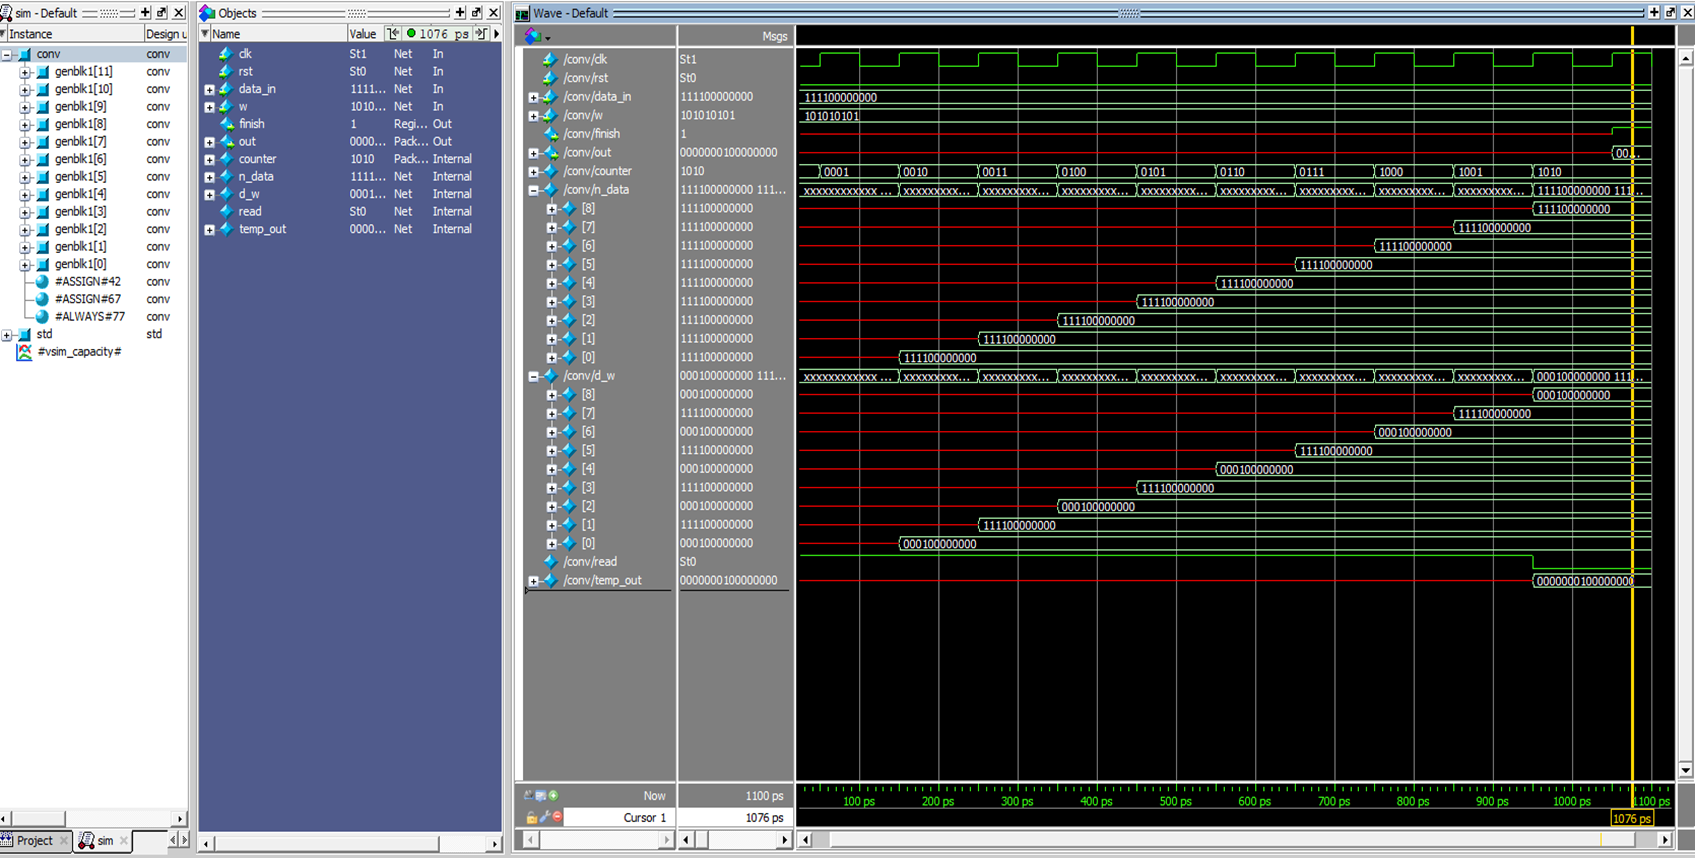
\includegraphics[width=0.9\linewidth]{Images/waveconv.png}
    \caption{Dạng sóng ngõ ra với testcase mixed weight với input bằng -1 (Q4.8)}
    \label{fig:enter-label}
\end{figure}
Quan sát thấy khí tín hiệu \textit{finish=1} kết quả ngõ ra bằng 1 (Q8.8) do ngõ vào cố định bằng -1 và với $weight=9'b101010101$ sẽ thực hiện 5 phép trừ và 4 phép cộng kết quả bằng 1 là chính xác. \\

VIết code testbench và sử dụng chức năng monitor của Modelsim để kiểm tra các testcase còn lại.
\begin{figure}[H]
    \centering
    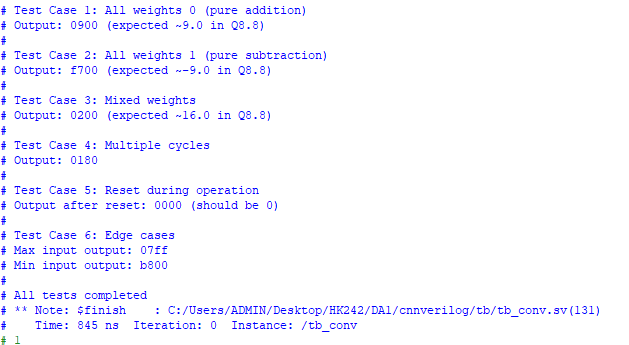
\includegraphics[width=0.75\linewidth]{Images/convtestcase.png}
    \caption{Testbench Conv}
    \label{fig:enter-label}
\end{figure}

\subsubsection{Synthesize}
Sử dụng phần mềm Gowin FPGA Designer để chạy synthesis ta có kết quả Netlist như hình \ref{fig:convsynth}.
\begin{figure}[H]
    \centering
    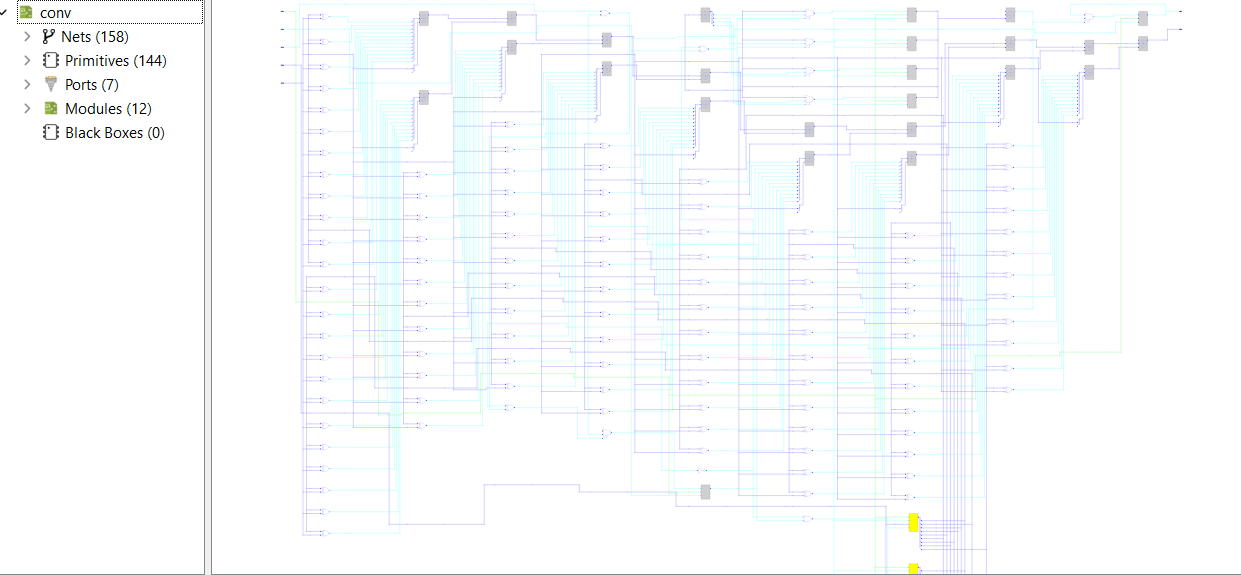
\includegraphics[width=0.75\linewidth]{Images/convsynth.png}
    \caption{Kết quả netlist synthesis khối Conv}
    \label{fig:convsynth}
\end{figure}

Ta có được báo cáo tài nguyên sử dụng và timing như sau.
\begin{table}[h]
\centering
\caption{Báo các sử dụng tài nguyên FPGA cho khối Conv}
\label{tab:resource_usage}
\begin{tabular}{
    l
    S[table-format=3.0]
    @{\hspace{1em}}
    S[table-format=4.0]
    S[table-format=1.1]
}
\toprule
\multirow{2}{*}{\textbf{Tài nguyên}} & 
\multicolumn{2}{c}{\textbf{Sử dụng/Tổng}} & 
\multirow{2}{*}{\textbf{Utilization}} \\
& \multicolumn{2}{c}{(đơn vị)} & \\
\midrule
Logic & 335 & (189 LUT, 128 ALU, 3 RAM16) / 8640 & 4.0\% \\
\hline
Register & \multicolumn{2}{l}{105 / 6693} & 2.0\% \\
\quad $\bullet$ Register as Latch & \multicolumn{2}{l}{0 / 6693} & 0.0\% \\
\quad $\bullet$ Register as FF & \multicolumn{2}{l}{105 / 6693} & 2.0\% \\
\hline
BSRAM & \multicolumn{2}{l}{0 / 26} & 0.0\% \\
\bottomrule
\end{tabular}

\vspace{0.5em}
\end{table}

\begin{figure}[H]
    \centering
    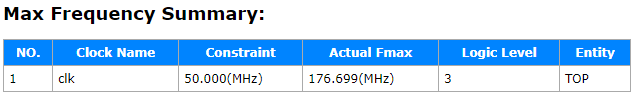
\includegraphics[width=0.9\linewidth]{Images/timingconv.png}
    \caption{Báo cáo timing khối Conv}
    \label{fig:enter-label}
\end{figure}

\subsection{Khối chuẩn hóa batch (Batch Nomalize)}
\subsubsection{Ý Tưởng Thiết Kế}
Nhắc lại phương trình tính Batch Normalize, mối quan hệ vào ra của dữ liệu được thể hiện qua công thức:
\begin{equation}
y_i = \gamma\frac{x_i-\mu}{\sqrt{\sigma^2}} + \beta
\end{equation}
Ta thấy khối này sử dụng 4 thông số trọng số, để giảm khói lượng tính toán và lưu trữ ta đơn giản phương trình như sau:
\begin{equation}
y_i = \gamma\frac{x_i-\mu}{\sqrt{\sigma^2}} + \beta = \theta x_i + \phi
\end{equation}
với:
\begin{itemize}
    \item $\theta = \gamma/\sqrt{\sigma^2}$ (hệ số tỷ lệ)
    \item $\phi = -\mu\gamma/\sqrt{\sigma^2} + \beta$ (hệ số dịch chuyển)
\end{itemize}

Với 2 hệ số $\theta$ và $\phi$ sẽ được tính toán trước và lượng tử hóa về kiểu dữ liệu Q4.8 do dựa theo khảo sát thì hệ số $\theta$ luôn dương và bé hơn 1 và hệ số $\phi$ của mô hình nằm trong khoảng kiểu dữ liệu Q4.8.
\begin{figure}[H]
    \centering
    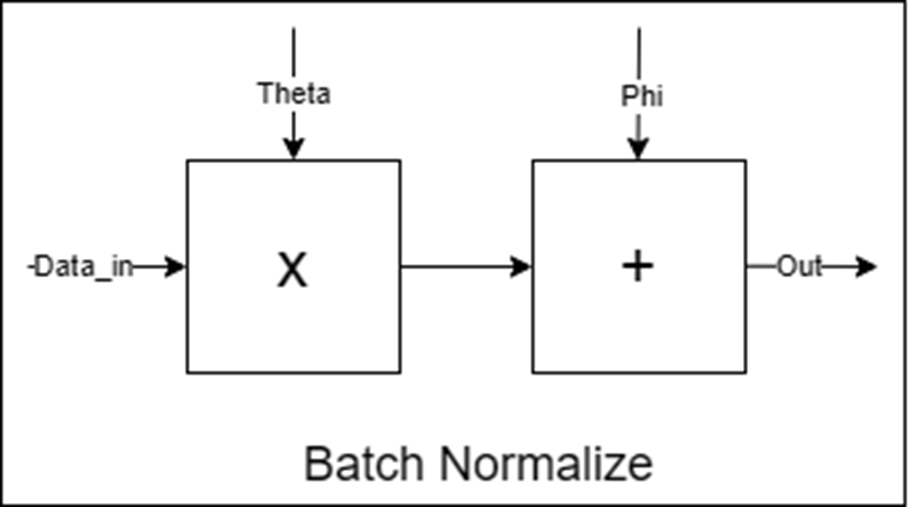
\includegraphics[width=0.5\linewidth]{Images/bnormblock.png}
    \caption{Sơ đồ khối Batch Nomalize}
    \label{fig:enter-label}
\end{figure}

\subsubsection{Thiết kế khối Batch Normalize}
\begin{table}[h]
\centering
\caption{Module BNORM Signal Definitions}
\label{tab:bnorm_signals}
\begin{tabular}{|>{\bfseries}l|l|l|l|}
\hline
\textbf{Signal Name} & \textbf{Direction} & \textbf{Width} & \textbf{Description} \\ \hline
clk      & Input  & 1  & System clock \\ \hline
rst      & Input  & 1  & Active-high reset \\ \hline
ready    & Input  & 1  & Data processing enable \\ \hline
data\_in & Input  & 16 & Input data (Q8.8 format) \\ \hline
theta    & Input  & 12 & Scale factor $\gamma/\sqrt{\sigma^2}$ \\ \hline
phi      & Input  & 12 & Shift factor $-\mu\gamma/\sqrt{\sigma^2} + \beta$ \\ \hline
finish   & Output & 1  & Operation completion flag \\ \hline
out      & Output & 12 & Result (Q4.8 format) \\ \hline
\end{tabular}
\end{table}

Bên trong khối này sẽ thực hiện tính toán ở kiểu dữ liệu Q8.8 sau đó cắt giảm 4 bit đầu để về kiểu dữ liệu Q4.8 và thực hiện luôn nhiệm vụ cuat lớp ReLU bằng cách kiểm tra bit MSB để quyết định kết quả ngõ ra. \\
\textbf{Các luồng tính toán chính}
\begin{itemize}
    \item Nhân với hệ số $\theta$:
    \begin{itemize}
        \item Mở rộng dấu ngõ vào 16-bit → 28-bit (Đảm bảo kết quả cho phép nhân có dấu 16-bit x 12-bit
        \item Nhân với $\theta$ (12-bit) sau khi mở rộng zero ($\theta$ luôn dương)
    \end{itemize}
    \item Cộng với hệ số $\phi$:
    \begin{itemize}
        \item Lấy 12 bit trung gian (bit 19-8) của kết quả nhân
        \item Cộng với hệ số dịch chuyển $\phi$
    \end{itemize}
    \item ReLU
    \begin{itemize}
        \item Phát hiện giá trị âm qua bit dấu (bit 11)
        \item Tự động cắt về 0 nếu âm (ReLU đơn giản)
    \end{itemize}
\end{itemize}
\textbf{Điều khiển trạng thái}
\begin{itemize}
    \item Tín hiệu \textit{finis}h được set sau 1 chu kỳ khi \textit{ready} active
    \item Reset đồng bộ thiết lập lại trạng thái
\end{itemize}

\subsubsection{Kiển thử \& Xác minh}

\begin{table}[h]
\centering
\caption{BNORM Module Verification Plan}
\label{tab:bnorm_verification}
\begin{tabular}{|l|l|l|}
\hline
\textbf{Test Category} & \textbf{Verification Method} & \textbf{Expected Result} \\ \hline
\multicolumn{3}{|c|}{\textbf{Reset Verification}} \\ \hline
Power-on reset & Assert reset, then release & All registers cleared, outputs zero \\ \hline
\multicolumn{3}{|c|}{\textbf{Basic Functionality}} \\ \hline
Identity transform & Set $\theta=1.0$, $\phi=0.0$ & Output = Input (Q4.8 scaled) \\ \hline
Scale only & Set $\theta=2.0$, $\phi=0.0$ & Output = 2 $\times$ Input \\ \hline
Shift only & Set $\theta=1.0$, $\phi=0.5$ & Output = Input + 0.5 \\ \hline
\multicolumn{3}{|c|}{\textbf{Boundary Cases}} \\ \hline
Max input value & Input 16'h7FFF (Q8.8) & Correct saturated output \\ \hline
Min input value & Input 16'h8000 (Q8.8) & Correct negative handling \\ \hline
Zero variance & Set $\theta=0.0$, $\phi=0.5$ & Output = 0.5 (constant) \\ \hline
\multicolumn{3}{|c|}{\textbf{Timing Control}} \\ \hline
Ready signal timing & Toggle ready during operation & Proper output only when ready=1 \\ \hline
Finish signal & Monitor finish signal & Asserted 2 cycles after ready \\ \hline
\multicolumn{3}{|c|}{\textbf{Reset Recovery}} \\ \hline
Mid-operation reset & Assert reset during calculation & Immediate termination, outputs zero \\ \hline
\end{tabular}
\end{table}

\begin{figure}[H]
    \centering
    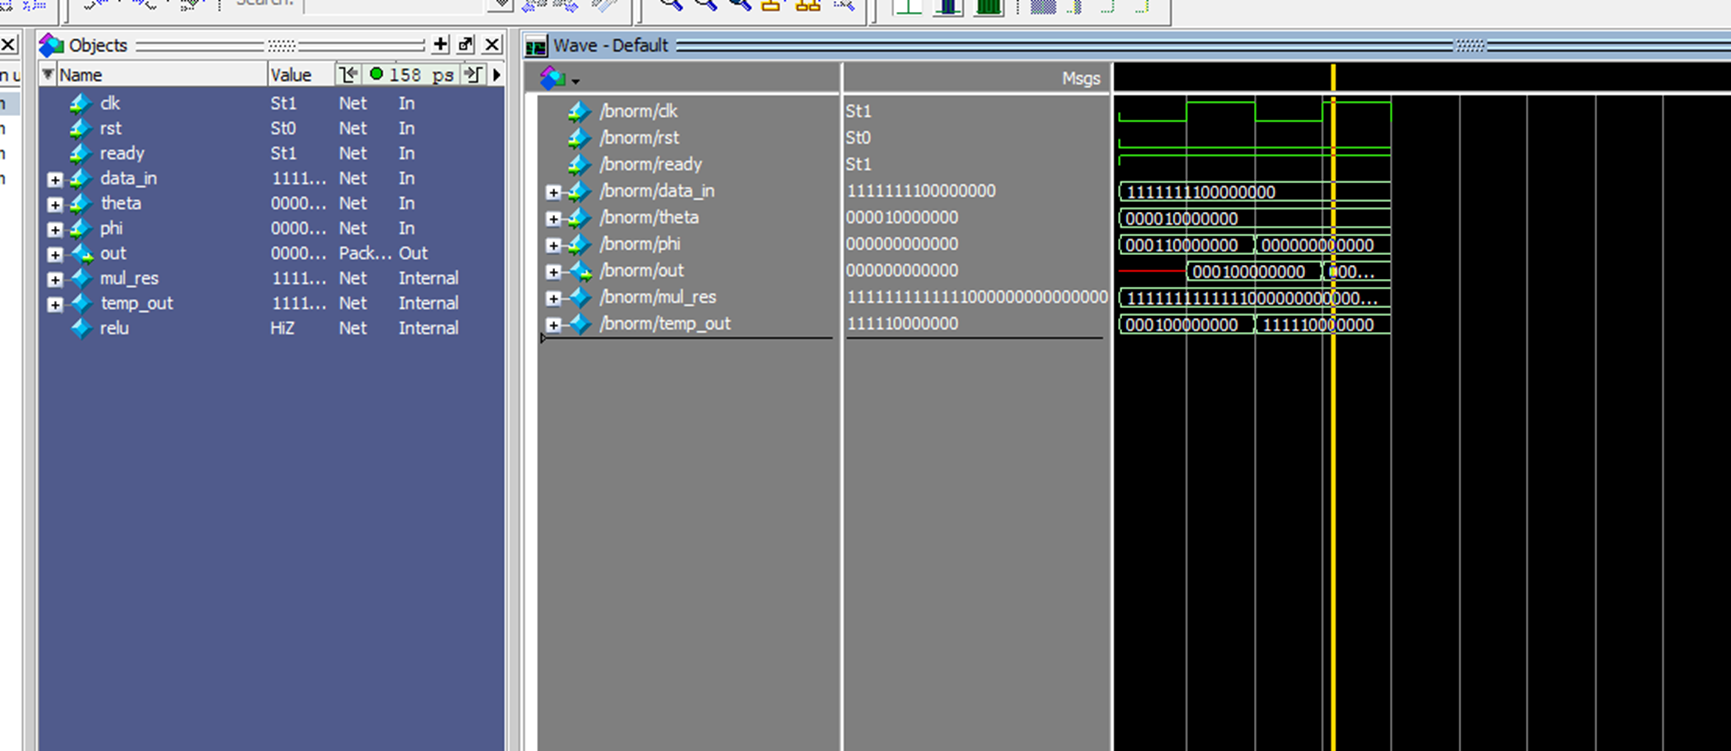
\includegraphics[width=0.75\linewidth]{Images/bnormtest.png}
    \caption{Dạng sóng ngõ ra với testcase Scale only với $\theta=1$ và ngõ vào bằng -1}
    \label{fig:enter-label}
\end{figure}
Quan sát khi tín hiệu \textit{finish=1} kết quả ngõ ra bằng -1 (Q4.8) do ngõ vào bằng -1 (Q8.8) với hệ số $\theta=1$ và $\phi=0$. \\
Viết code testbench và sử dụng chức năng monitor của Modelsim để kiểm tra các testcase
còn lại.

\begin{figure}[H]
    \centering
    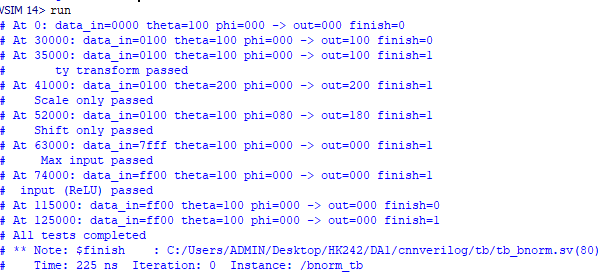
\includegraphics[width=0.75\linewidth]{Images/bnormtst.png}
    \caption{Testbench Bnorm}
    \label{fig:enter-label}
\end{figure}

\subsubsection{Synthesize}
Sử dụng phần mềm Gowin FPGA Designer để chạy synthesis ta có kết quả Netlist như hình \ref{fig:bnormsynth}.
\begin{figure}[H]
    \centering
    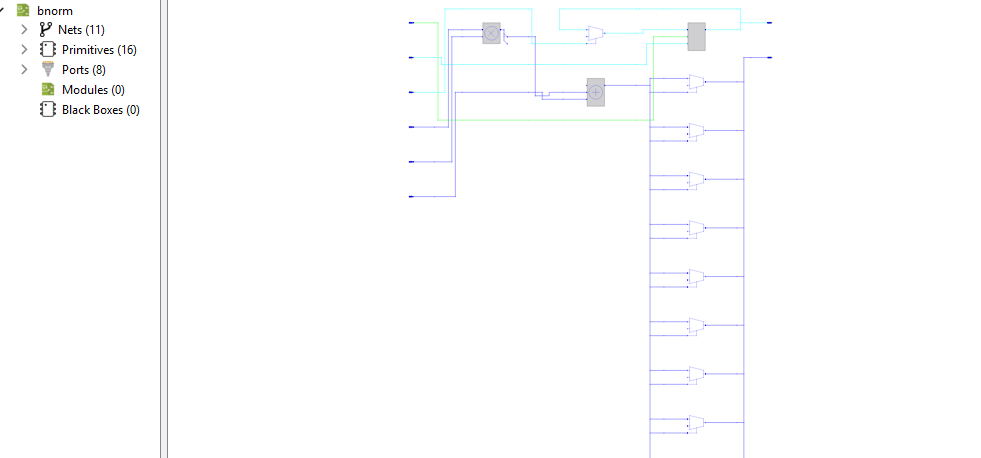
\includegraphics[width=0.75\linewidth]{Images/bnsynth.png}
    \caption{Kết quả netlist synthesis khối Bnorm}
    \label{fig:bnormsynth}
\end{figure}
Ta có được báo cáo tài nguyên sử dụng như sau.

\begin{table}[h]
\centering
\caption{Báo các sử dụng tài nguyên FPGA cho khối Bnorm}
\label{tab:resource_usage}
\begin{tabular}{
    l
    S[table-format=3.0]
    @{\hspace{1em}}
    S[table-format=4.0]
    S[table-format=1.1]
}
\toprule
\multirow{2}{*}{\textbf{Tài nguyên}} & 
\multicolumn{2}{c}{\textbf{Sử dụng/Tổng}} & 
\multirow{2}{*}{\textbf{Utilization}} \\
& \multicolumn{2}{c}{(đơn vị)} & \\
\midrule
Logic & 23 & (11 LUT, 12 ALU) / 8640 & <1.0\% \\
\hline
Register & \multicolumn{2}{l}{1 / 6693} & <1.0\% \\
\quad $\bullet$ Register as Latch & \multicolumn{2}{l}{0 / 6693} & 0.0\% \\
\quad $\bullet$ Register as FF & \multicolumn{2}{l}{1 / 6693} & <1.0\% \\
\hline
BSRAM & \multicolumn{2}{l}{0 / 26} & 0.0\% \\
\hline
DSP &  &  \\
\quad $\bullet$ MULT18X18 & \multicolumn{2}{l}{1} &  \\
\bottomrule
\end{tabular}

\vspace{0.5em}
\end{table}

\subsection{Khối Maxpool}
\subsubsection{Ý Tưởng Thiết Kế}
So sánh lần lượt các giá trị 12-bit (Q4.8) không cần để ý đến dấu. Nếu có giá trị lớn hơn giá trị temp thì sẽ thay thế temp bằng giá trị đó. Nếu có tín hiệu \textit{end} sẽ kết thúc quá trình so sánh và bật cờ $finish$. Có thể sử dụng khối này dùng cho quá trình Max pooling hoặc Global pooling.

\subsubsection{Thiết kế khối Maxpool}
\begin{table}[H]
\centering
\caption{Module MaxPool Signal Definitions}
\begin{tabular}{>{\ttfamily}l l l p{6cm}}
\toprule
\textbf{Signal Name} & \textbf{Direction} & \textbf{Width} & \textbf{Description} \\
\midrule
clk      & Input  & 1  & System clock \\
rst      & Input  & 1  & Active-high reset \\
data\_in & Input  & 12 & Input data (Q4.8 format) \\
end\_data & Input & 1  & End of input data flag \\
\midrule
finish   & Output & 1  & Operation completion flag \\
out      & Output & 12 & Max pooling result (Q4.8 format) \\
\bottomrule
\end{tabular}
\end{table}

Thiết kế khối Maxpool theo flow sau bằng ngôn ngữ verilog.
\begin{figure}[H]
    \centering
    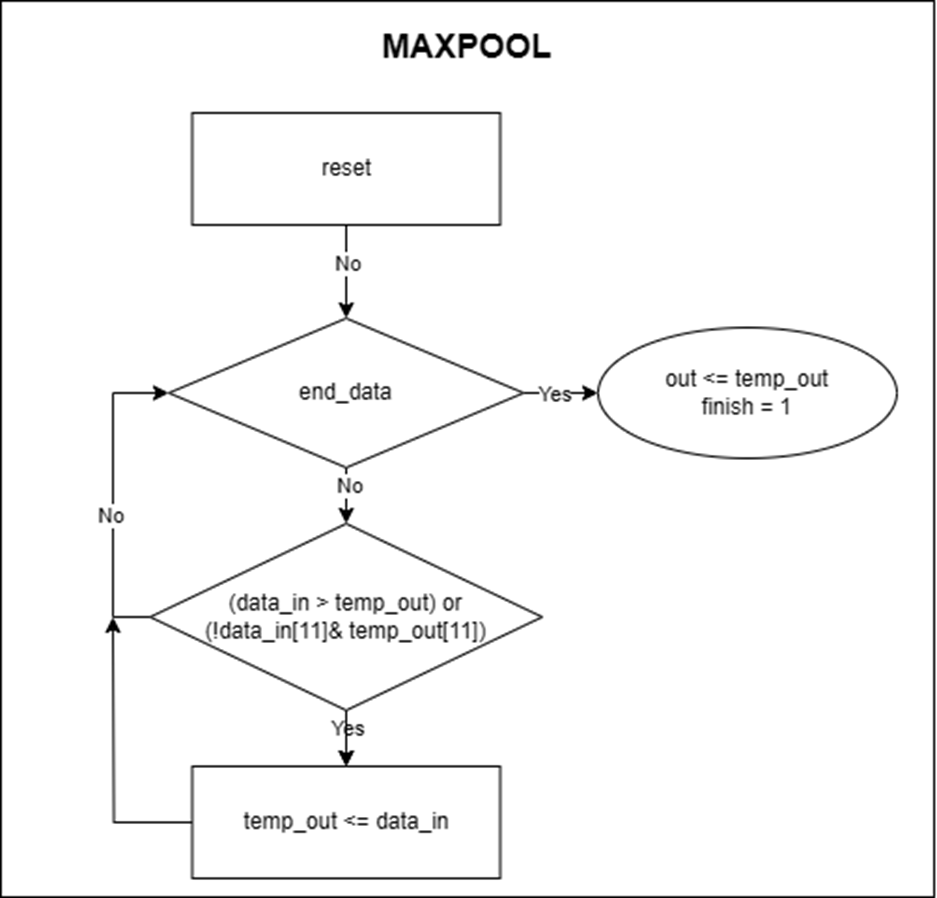
\includegraphics[width=0.75\linewidth]{Images/mpflow.png}
    \caption{Maxpool flow chart}
    \label{fig:enter-label}
\end{figure}

\subsubsection{Kiển thử \& Xác minh}

\begin{table}[h]
\centering
\caption{MaxPool Module Verification Plan}
\label{tab:maxpool_verification}
\begin{tabular}{|l|l|l|}
\hline
\textbf{Test Category} & \textbf{Verification Method} & \textbf{Expected Result} \\ \hline
\multicolumn{3}{|c|}{\textbf{Reset Verification}} \\ \hline
Power-on reset & Assert reset, then release & All registers cleared, outputs zero \\ \hline
Mid-operation reset & Assert reset during window processing & Immediate output reset to zero \\ \hline
\multicolumn{3}{|c|}{\textbf{Basic Functionality}} \\ \hline
Single 2x2 window & Input [1.0, 0.5, 1.5, 0.0] (Q4.8) & Output = 1.5 (max value) \\ \hline

Identical values & Input [0.8, 0.8, 0.8, 0.8] & Output = 0.8 (any duplicate accepted) \\ \hline
\multicolumn{3}{|c|}{\textbf{Boundary Cases}} \\ \hline
Max Q4.8 value & Input [7.996, 0.0, 0.0, 0.0] (16'h7FF) & Output = 7.996 \\ \hline

\multicolumn{3}{|c|}{\textbf{Timing Control}} \\ \hline
end\_data timing & Toggle end\_data during streaming & finish asserts 1 cycle after last window \\ \hline
Data starvation & Delay between input windows & Correct output timing with gaps \\ \hline
\multicolumn{3}{|c|}{\textbf{Error Cases}} \\ \hline
Incomplete window & Send 3 values then end\_data & Output remains zero (no false trigger) \\ \hline
\end{tabular}
\end{table}


\begin{figure}[H]
    \centering
    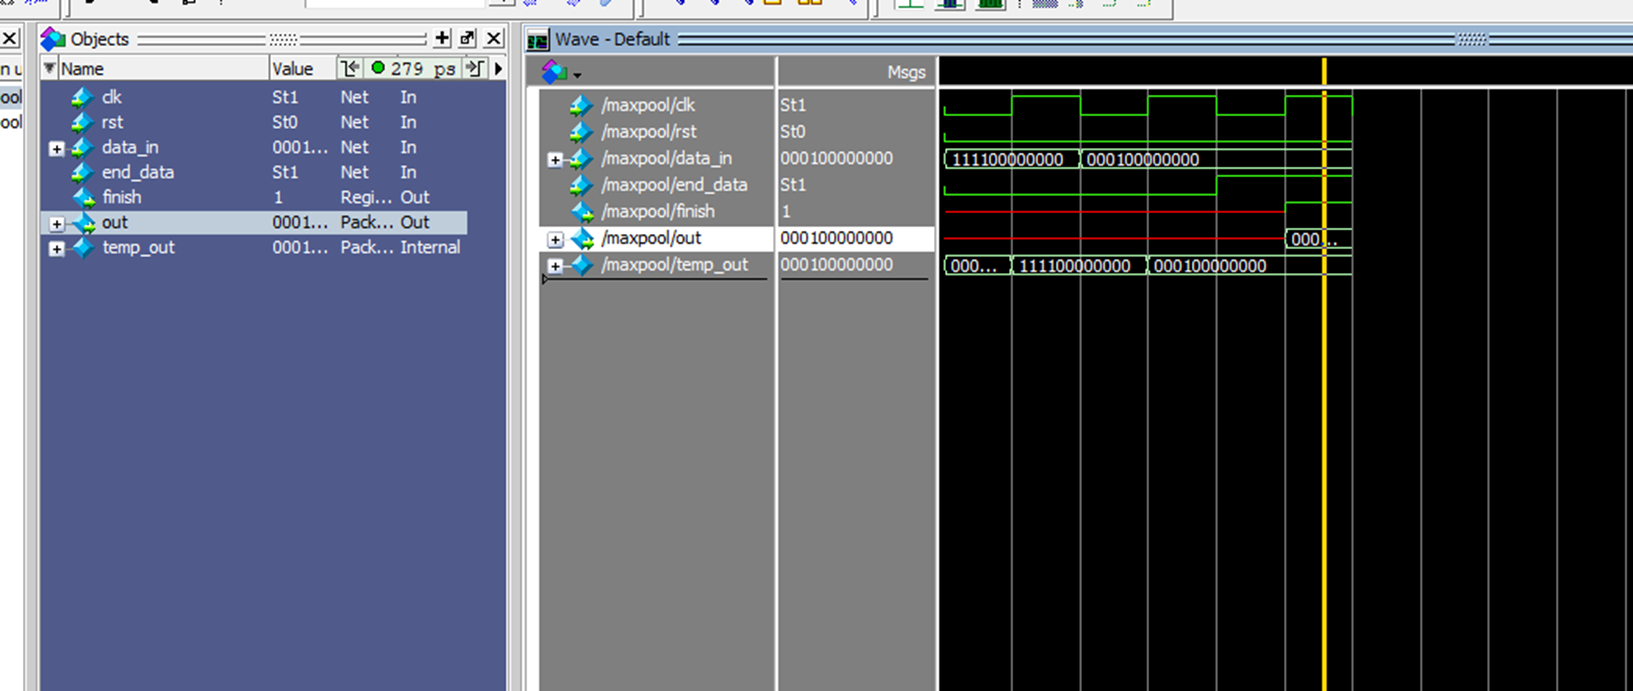
\includegraphics[width=0.9\linewidth]{Images/tbmp.png}
    \caption{Dạng sóng ngõ ra cho testcase chức năng chính khối maxpool}
    \label{fig:enter-label}
\end{figure}
Quan sát khi tín hiệu \textit{finish=1} kết quả ngõ ra bằng 1 (Q4.8) do ngõ vào lần lượt bằng -1 và 1 sau khi cờ \textit{end\_data} được bật sẽ bật cờ \textit{finish} và trả kết quả ngõ ra bằng 1. \\
Viết code testbench và kiểm tra dạng sóng các testcase còn lại.


\subsubsection{Synthesize}
Sử dụng phần mềm Gowin FPGA Designer để chạy synthesis ta có kết quả Netlist như hình \ref{fig:mpsynth}.
\begin{figure}[H]
    \centering
    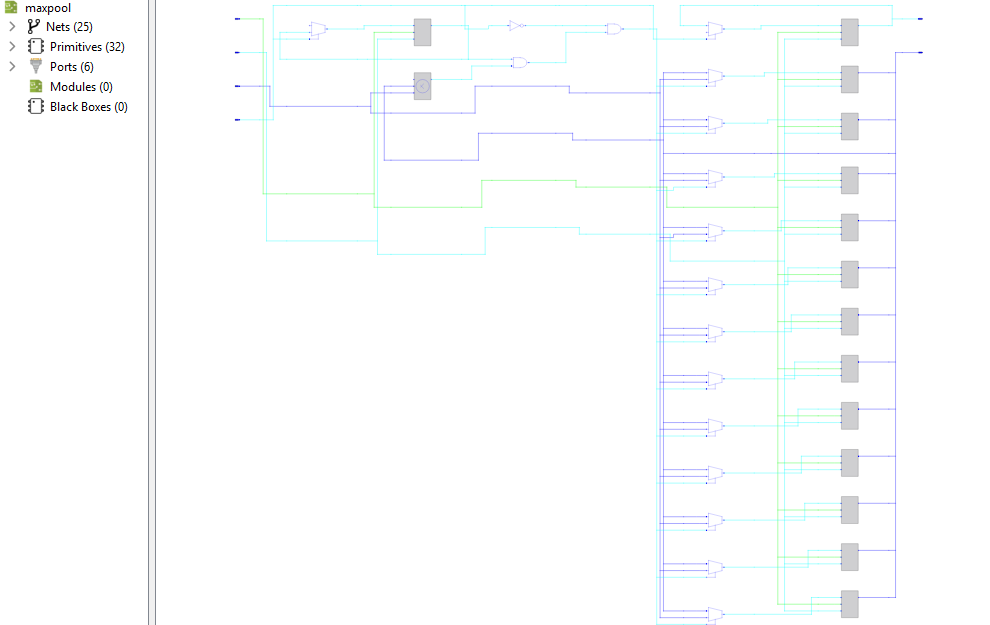
\includegraphics[width=0.75\linewidth]{Images/mpnet.png}
    \caption{Kết quả netlist synthesis khối Maxpool}
    \label{fig:mpsynth}
\end{figure}
Ta có được báo cáo tài nguyên sử dụng và timing như sau.

\begin{table}[H]
\centering
\caption{Báo các sử dụng tài nguyên FPGA cho khối Maxpool}
\label{tab:resource_usage}
\begin{tabular}{
    l
    S[table-format=3.0]
    @{\hspace{1em}}
    S[table-format=4.0]
    S[table-format=1.1]
}
\toprule
\multirow{2}{*}{\textbf{Tài nguyên}} & 
\multicolumn{2}{c}{\textbf{Sử dụng/Tổng}} & 
\multirow{2}{*}{\textbf{Utilization}} \\
& \multicolumn{2}{c}{(đơn vị)} & \\
\midrule
Logic & 14 & (2 LUT, 12 ALU) / 8640 & <1.0\% \\
\hline
Register & \multicolumn{2}{l}{14 / 6693} & <1.0\% \\
\quad $\bullet$ Register as Latch & \multicolumn{2}{l}{0 / 6693} & 0.0\% \\
\quad $\bullet$ Register as FF & \multicolumn{2}{l}{14 / 6693} & <1.0\% \\
\hline
BSRAM & \multicolumn{2}{l}{0 / 26} & 0.0\% \\
\hline
\bottomrule
\end{tabular}

\begin{figure}[H]
    \centering
    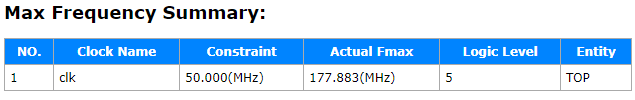
\includegraphics[width=0.9\linewidth]{Images/mptime.png}
    \caption{Báo cáo timing khối Maxpool}
    \label{fig:enter-label}
\end{figure}

\vspace{0.5em}
\end{table}

\subsection{Khối Fully Connect}
\subsubsection{Ý Tưởng Thiết Kế}
\begin{itemize}
    \item Thiết kế bộ fully connected layer tối ưu cho bài toán phân lớp 10 lớp:
    \begin{itemize}
        \item Đầu vào dạng fixed-point Q4.8 (12-bit)
        \item Trọng số dạng Q4.8 (12-bit)
        \item Đầu ra dạng one-hot 4-bit (10 lớp)
        \item Hỗ trợ batch size lên đến 16 mẫu (counter 4-bit)
    \end{itemize}
    
    \item Kết hợp 2 module chính:
    \begin{itemize}
        \item \textit{Multiply-Accumulate (MAC):} 10 bộ MAC song song cho 10 lớp đầu ra
        \item \textit{Max Tournament:} Cây so sánh 5 tầng để tìm lớp có giá trị lớn nhất
    \end{itemize}
    \begin{figure}[H]
        \centering
        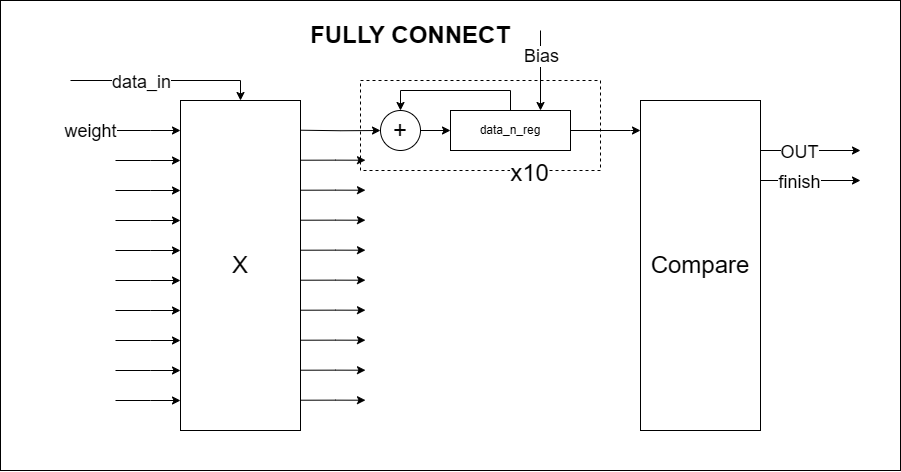
\includegraphics[width=0.8\linewidth]{Images/fc_arch.png}
        \caption{Sơ đồ khối FullyConnect với pipeline 3 giai đoạn}
        \label{fig:fc_arch}
    \end{figure}

    \begin{figure}[H]
        \centering
        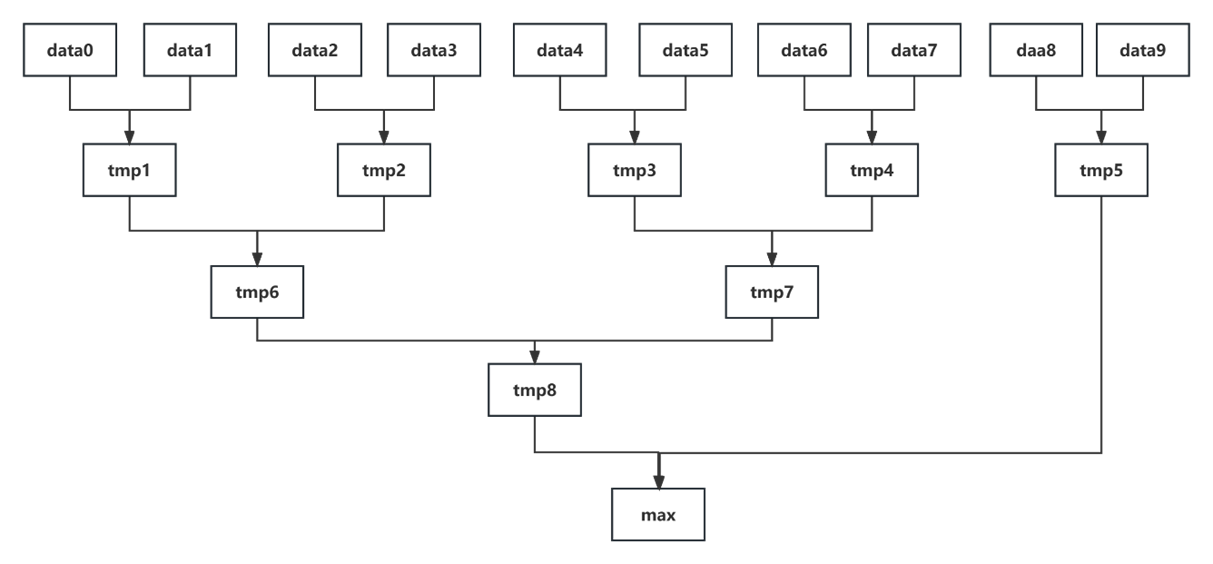
\includegraphics[width=0.8\linewidth]{Images/comptree.png}
        \caption{Sơ đồ khối cây so sánh 5 tầng}
        \label{fig:enter-label}
    \end{figure}

    \item Cơ chế pipeline:
    \begin{itemize}
        \item Stage 1 (Compute): Nhân-ma-trận và cộng bias từ ROM (1 chu kỳ)
        \item Stage 2 (Vote): So sánh 10 giá trị dense qua cây tournament (3 chu kỳ)
    \end{itemize}

    \item Triển khai phép toán signed MAC:
    \begin{verbatim}
        // Signed multiplication with sign extension
        mul_res[i] = {12'b0, data_in} * {{12{w[i][11]}}, w[i]}; 
        // Accumulation with 16-bit bias
        dense_temp[i] = dense[i] + mul_res[i][23:8];
    \end{verbatim}

    \item Tối ưu hóa phần cứng:
    \begin{itemize}
        \item Sử dụng DSP blocks cho phép nhân 12-bit thay vì LUT
        \item Shared weight loading qua SIPO110 tiết kiệm 78\% bus điều khiển
    \end{itemize}
\end{itemize}

\subsubsection{Thiết kế khối FullyConnect}
\begin{table}[H]
\centering
\caption{Module FullyConnect Signal Definitions}
\label{tab:fc_signals}
\begin{tabular}{llll}
\toprule
\textbf{Signal Name} & \textbf{Direction} & \textbf{Width} & \textbf{Description} \\
\midrule
clk & Input & 1 & System clock \\
rst & Input & 1 & Active-high reset \\
data\_in & Input & 12 & Input feature map (Q4.8) \\
w & Input & 120 & Weight value (Q4.8) \\
pos\_data & Output & 4 & Position counter \\
load\_weight & Output & 1 & Weight loading flag \\
cnn\_out & Output & 4 & Classification result \\
finish & Output & 1 & Operation completion flag \\
\bottomrule
\end{tabular}
\end{table}

\begin{itemize}
    \item Cơ chế hoạt động:
    \begin{itemize}
        \item Giai đoạn tính toán:
        \begin{itemize}
            \item Thực hiện phép nhân có dấu Q4.8 $\times$ Q4.8
            \item Cộng dồn với bias pre-load từ bộ nhớ ROM
            \item Pipeline 3 giai đoạn: Nhân $\rightarrow$ Cộng $\rightarrow$ So sánh
        \end{itemize}
        \item Giai đoạn voting:
        \begin{itemize}
            \item So sánh 10 giá trị dense theo cơ chế tournament sort
            \item Xuất kết quả lớp có giá trị lớn nhất (4-bit one-hot)
        \end{itemize}
    \end{itemize}
    
    \item Kiến trúc Pipeline:
    \begin{itemize}
        \item Stage 1: 10 bộ nhân song song (12-bit $\times$ 12-bit)
        \item Stage 2: 10 bộ cộng có dấu 16-bit với bias
        \item Stage 3: Cây so sánh 5 tầng để tìm max
    \end{itemize}
\end{itemize}

\subsubsection{Kiểm Thử \& Xác Minh}
\begin{table}[H]
\centering
\caption{FullyConnect Verification Plan}
\begin{tabular}{>{\bfseries}p{2.5cm}p{4cm}p{4cm}p{3cm}}
\toprule
\textbf{Test Category} & \textbf{Test Case} & \textbf{Verification Method} & \textbf{Expected Result} \\
\midrule
Reset Verification & Power-on reset & Assert reset, then release & All registers cleared, cnn\_out=15 \\
\hline
Weight Loading & Serial weight shifting & Input known weight pattern & Correct parallel output after 12 cycles \\
\hline
Basic Inference & All weights=1.0 & Input fixed value 1.0 & Correct dense[i] = bias[i] + 1.0 \\
\hline
Boundary Cases & Max Q4.8 input (7.996) & Input 12'h7FF with random weights & Proper saturated accumulation \\
\hline
Negative Values & Mixed sign weights & Alternate positive/negative weights & Correct signed arithmetic \\
\hline
Timing Control & Finish signal timing & Monitor pos\_data counter & finish=1 when pos\_data overflows \\
\hline
Comparison Logic & All dense equal & Set identical dense values & Any class selected (one-hot) \\
\hline
Bias Loading & ROM initialization & Check initial dense values & Match predefined biasrom.mem \\
\bottomrule
\end{tabular}
\end{table}

\begin{figure}[H]
    \centering
    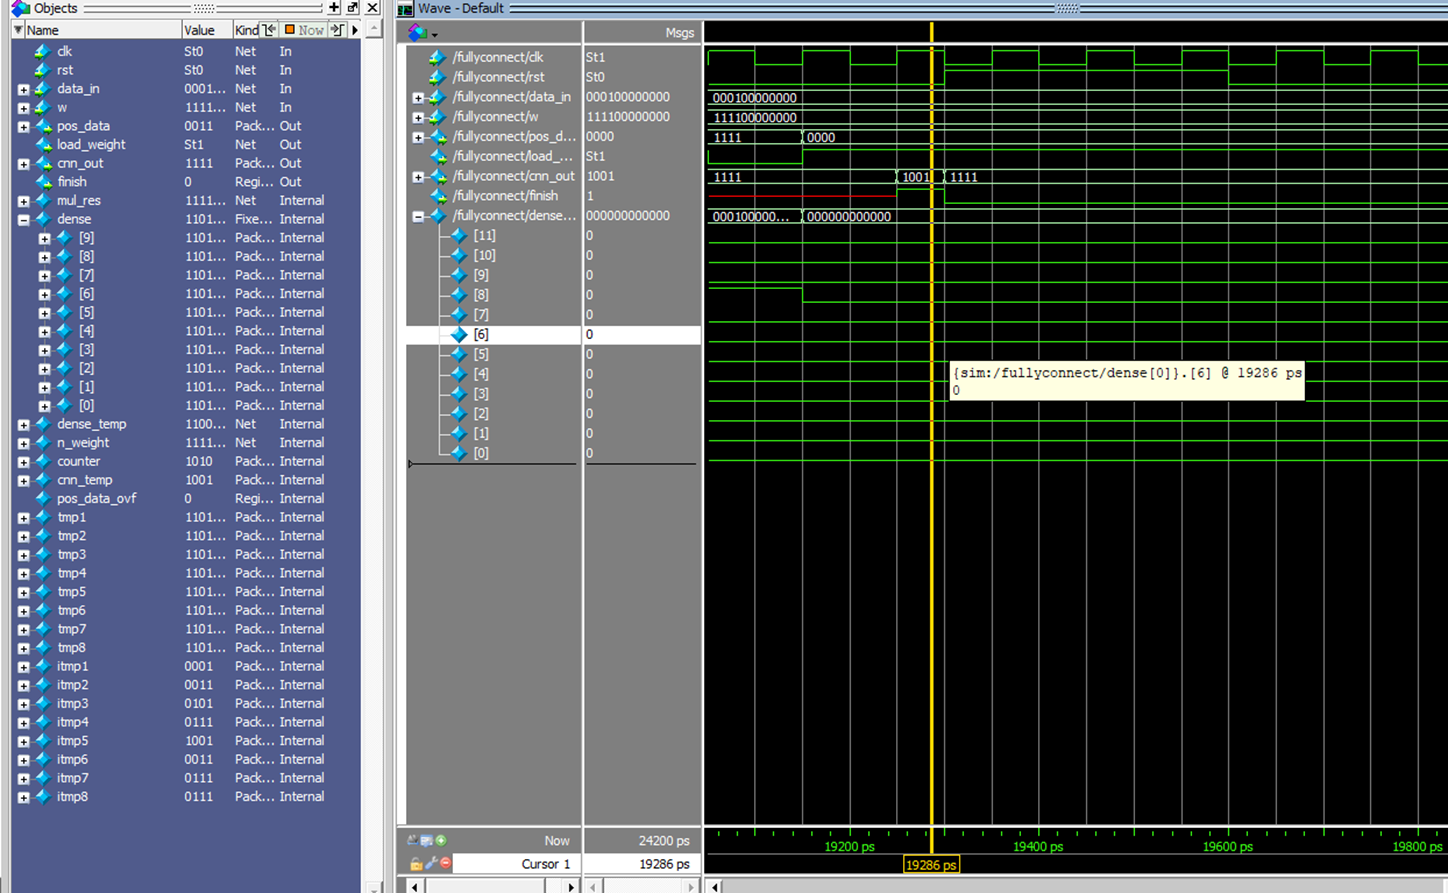
\includegraphics[width=0.9\linewidth]{Images/wavefc.png}
    \caption{Dạng sóng testbench với tất cả giá trị dense giống nhau}
    \label{fig:fc_wave}
\end{figure}
Với tất cả giá trị dense giống nhau khi đưa vào cây so sánh theo thuật toán cây so sánh nếu tất cả các giấ trị so sánh bằng nhau kết quả trả về sẽ là 9. \\
Viết code testbench và sử dụng chức năng monitor của Modelsim để kiểm tra các testcase
còn lại.

\begin{figure}[H]
    \centering
    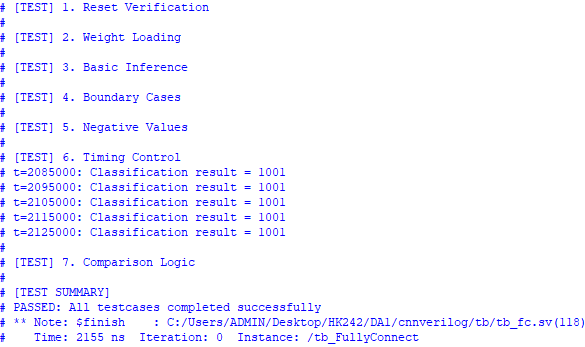
\includegraphics[width=0.75\linewidth]{Images/tbfc.png}
    \caption{Testbench Fully Connect}
    \label{fig:enter-label}
\end{figure}

\subsubsection{Synthesize}
Sử dụng phần mềm Gowin FPGA Designer để chạy synthesis ta có kết quả Netlist như hình \ref{fig:fc_synth}.
\begin{figure}[H]
    \centering
    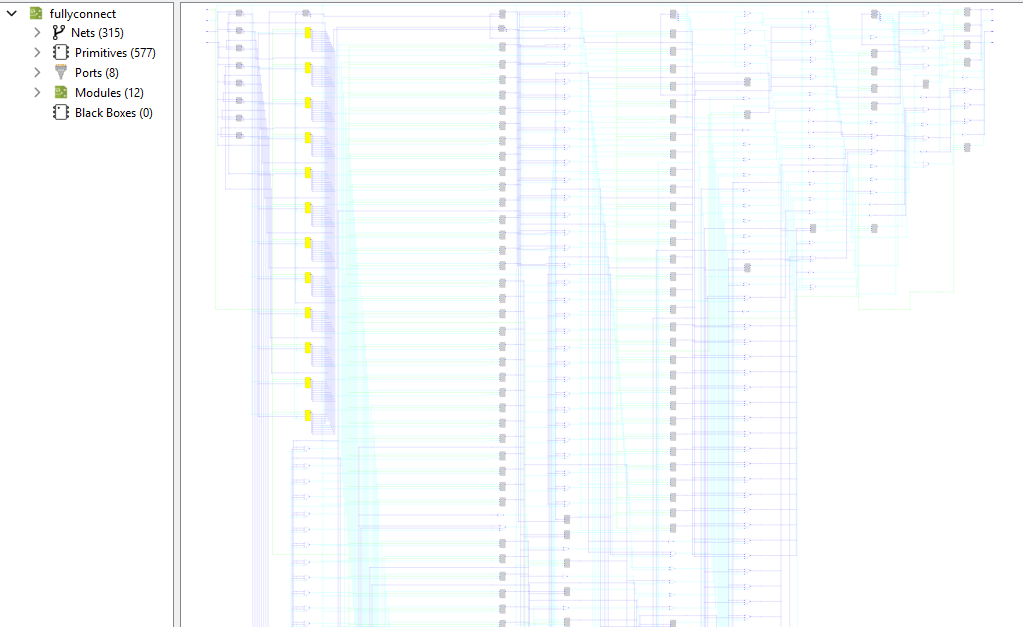
\includegraphics[width=0.75\linewidth]{Images/fcsynth.png}
    \caption{Kết quả netlist synthesis khối FullyConnect}
    \label{fig:fc_synth}
\end{figure}

Ta có được báo cáo tài nguyên sử dụng và timing như sau.

\begin{table}[h]
\centering
\caption{Báo cáo tài nguyên FPGA cho FullyConnect}
\label{tab:fc_resource}
\begin{tabular}{
    l
    S[table-format=3.0]
    @{\hspace{1em}}
    S[table-format=4.0]
    S[table-format=2.1]
}
\toprule
\multirow{2}{*}{\textbf{Tài nguyên}} & 
\multicolumn{2}{c}{\textbf{Sử dụng/Tổng}} & 
\multirow{2}{*}{\textbf{Utilization}} \\
& \multicolumn{2}{c}{(đơn vị)} & \\
\midrule
Logic & 550 & (310 LUT, 240 ALU) / 8640 & 7.0\% \\
\hline
Register & \multicolumn{2}{l}{182 / 6693} & 3.0\% \\
\quad $\bullet$ FF & \multicolumn{2}{l}{0 / 6693} & 0\% \\
\quad $\bullet$ Latch & \multicolumn{2}{l}{182 / 6693} & 3.0\% \\
\hline
DSP &  &  \\
\quad $\bullet$ MULT18X18 & 10 &  \\
\bottomrule
\end{tabular}
\end{table}

\begin{figure}[H]
    \centering
    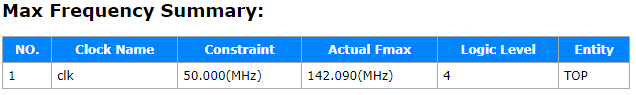
\includegraphics[width=0.9\linewidth]{Images/timingfc.png}
    \caption{Báo cáo timing khối Fully Connect}
    \label{fig:fc_timing}
\end{figure}

\subsection{Khối BSRam}

Ta sẽ phân vùng Ram như sau để lưu dữ liệu từng lớp.
\begin{table}[H]
\centering
\caption{Bảng memory map hệ thống CNN (14-bit địa chỉ, 12-bit dữ liệu)}
\label{tab:memory_map}
\begin{tabular}{|>{\ttfamily}c|>{\ttfamily}c|>{\ttfamily}c|l|}
\hline
\rowcolor{gray!20}
\textbf{Vùng} & \textbf{Địa chỉ bắt đầu} & \textbf{Kích thước} & \textbf{Mô tả} \\
\hline
% \rowcolor{convcolor}
PADDING & 14'd0 & 1 words & \multirow{2}{8cm}{Chứa zero dùng để làm padding cho CONV} \\
       & (0x0000) & (0x0001) & \\
\hline

\rowcolor{convcolor}
CONV1 & 14'd1 & 784 words & \multirow{2}{8cm}{Chứa dữ liệu 1 ảnh 28x28 đầu vào CONV1} \\
       & (0x0001) & (0x0310) & \\
\hline
\rowcolor{convcolor}
CONV2 & 14'd785 & 3136 words & \multirow{2}{8cm}{Chứa dữ liệu 4 ảnh 28x28 đầu vào CONV2} \\
       & (0x0311) & (0x0C40) & \\
\hline
\rowcolor{poolcolor}
MPOOL1 & 14'd3921 & 3136 words & Chứa dữ liệu 4 ảnh 28x28 đầu vào MPOOL1 \\
       & (0x0F51) & (0x0C40) & \\
\hline
\rowcolor{convcolor}
CONV3 & 14'd7057 & 784 words & Chứa dữ liệu 4 ảnh 14x14 đầu vào CONV3 \\
       & (0x1B91) & (0x0310) & \\
\hline
\rowcolor{convcolor}
CONV4 & 14'd7841 & 1568 words & Chứa dữ liệu 8 ảnh 14x14 đầu vào CONV4 \\
       & (0x1EA1) & (0x0620) & \\
\hline
\rowcolor{poolcolor}
MPOOL2 & 14'd9409 & 1568 words & Chứa dữ liệu 8 ảnh 14x14 đầu vào MPOOl2 \\
       & (0x24C1) & (0x0620) & \\
\hline
\rowcolor{convcolor}
CONV5 & 14'd10977 & 392 words & Chứa dữ liệu 8 ảnh 7x7 đầu vào CONV5 \\
       & (0x2AE1) & (0x0188) & \\
\hline
\rowcolor{poolcolor}
GMPOOL & 14'd11369 & 784 words & Chứa dữ liệu 16 ảnh 7x7 đầu vào GMPOOL \\
       & (0x2C69) & (0x0310) & \\
\hline
\rowcolor{densecolor}
DENSE & 14'd12153 & 16 words & Chứa dữ liệu 16 ảnh 1x1 đầu vào Fully Connect \\
       & (0x2F79) & (0x0010) & \\
\hline
TỔNG &  & 12169 words &  \\

\hline
\end{tabular}
\end{table}

Như vậy để có thể lưu trữ được tất cả dữ liệu cần thiết cho nhận diện số viết tay ta cần dùng bộ nhớ ram có kích thước khoảng 18kByte.
\begin{figure}[H]
    \centering
    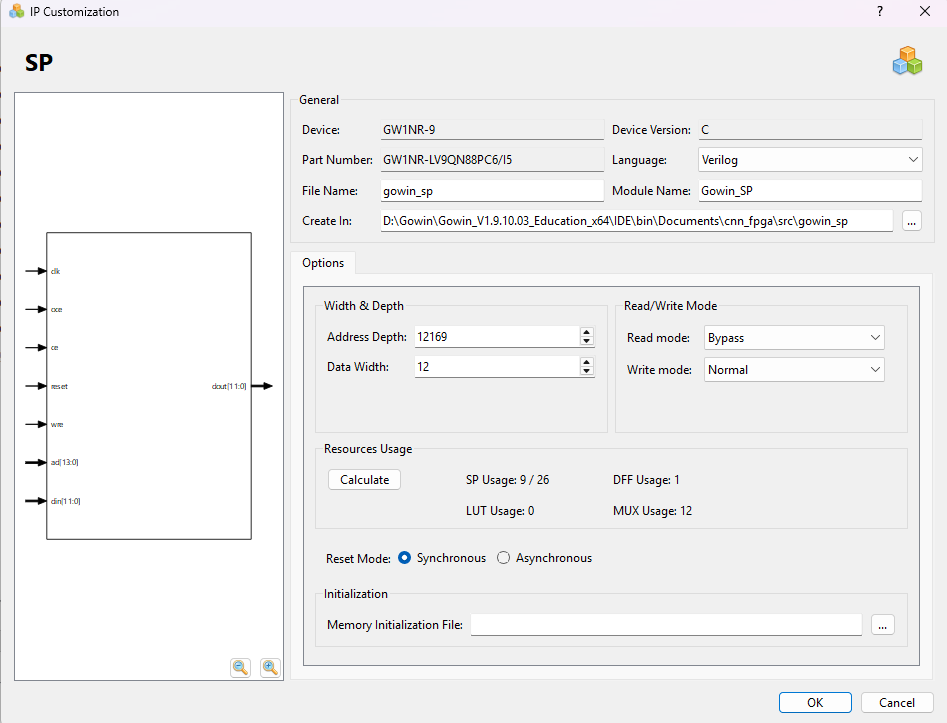
\includegraphics[width=0.75\linewidth]{Images/ipcoreram.png}
    \caption{BSRam ip core Gowin}
    \label{fig:enter-label}
\end{figure}
Để đơn giản việt thiết kế ta có thưeer dùng tính năng IP Core của tool Gowin để tạo khối BSRAM. Kit Tang Nano 9K hỗ trợ đến 26 khối BSRAM với kích thước mỗi khối là 16kBit. Theo hình ta thấy cần sử dụng 9 khối BSRAM tương ứng với 18kByte như tính toán bên trên.

\subsection{Các khối ROM chứa dữ liệu trọng số}
Triển khai mô hình AI trên phần cứng đòi hỏi chuyển đổi trọng số từ định dạng dấu phẩy động (float32) sang định dạng cố định (fixed-point) Q4.8 và nhị phân của lớp convolution. File .mem trong Verilog chứa dữ liệu nhị phân/hex, được sử dụng để khởi tạo bộ nhớ ROM/RAM.

\begin{figure}[H]
    \centering
    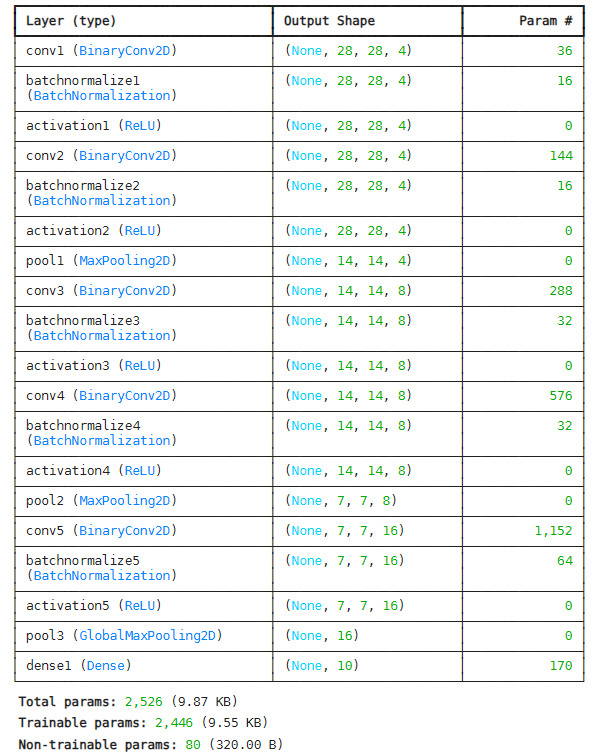
\includegraphics[width=0.75\linewidth]{Images/cnnmodel.png}
    \caption{Báo cáo trọng số từng lớp CNN}
    \label{fig:enter-label}
\end{figure}

\textbf{Các bước thực hiện}
\begin{itemize}
    \item B1: Trích xuất Trọng số từ CNN bằng cách sử dụng API của TensorFlow ( \texttt{model.layers[i].get\_weights()}).
    \item B2: Chuyển đổi sang Nhị phân
    \begin{itemize}
        \item Làm phẳng (flatten) filter 3x3 và chuyển đổi trọng số của lớp conv về dạng nhị phân ta được một chuối 9-bit tương ứng với 9 trọng số của filter 3x3.
        \item Tính toán trước hệ số $\theta$ và $\phi$ mà ta thiết kế theo 4 hệ số trọng số $\alpha,\beta,\gamma,\mu$ của lớp Batch Normalize và lượng tử vệ đinh dạng Q4.8.
        \item Lượng tử trọng số và bias của lớp fully connect về dạng Q4.8.
    \end{itemize}
    \item B3: Tạo File .mem cho Verilog
    \item B4: Khởi tạo bộ nhớ trong Verilog với từng khối ROM.
\end{itemize}
\textbf{Kích thước Rom}
\begin{itemize}
    \item Tổng các param của lớp conv là: $36+144+288+576+1152=2196$. Vậy ta cần 1 ROM chứa 244x9-bit để lưu trọng số lớp conv.
    \item Tổng các param của lớp batch normalize là: $16+16+32+32+64=160$ do ta đã giảm một nửa số param của lớp này nên còn 80 param. Vậy ta cần 1 ROM chứa 80x12-bit để lưu trọng số lớp Batch normalize.
    \item Tổng số param của lớp fully connect là 170 bỏ qua 10 trọng số bias được load sẵn ta cần 1 ROM chứa 160x12-bit để lưu trọng số lớp này.
\end{itemize}



\subsection{Khối điều khiển (FSM)}
\subsubsection{Tổng quan}
Dựa theo flow tính toán và sơ đồ của mạng CNN ta lập được một sơ đồ máy trạng thái như sau (Gộp 3 lớp BinaryConv + BatchNormalize + ReLU thành 1 trạng hái CONV):

\begin{figure}[H]
    \centering
    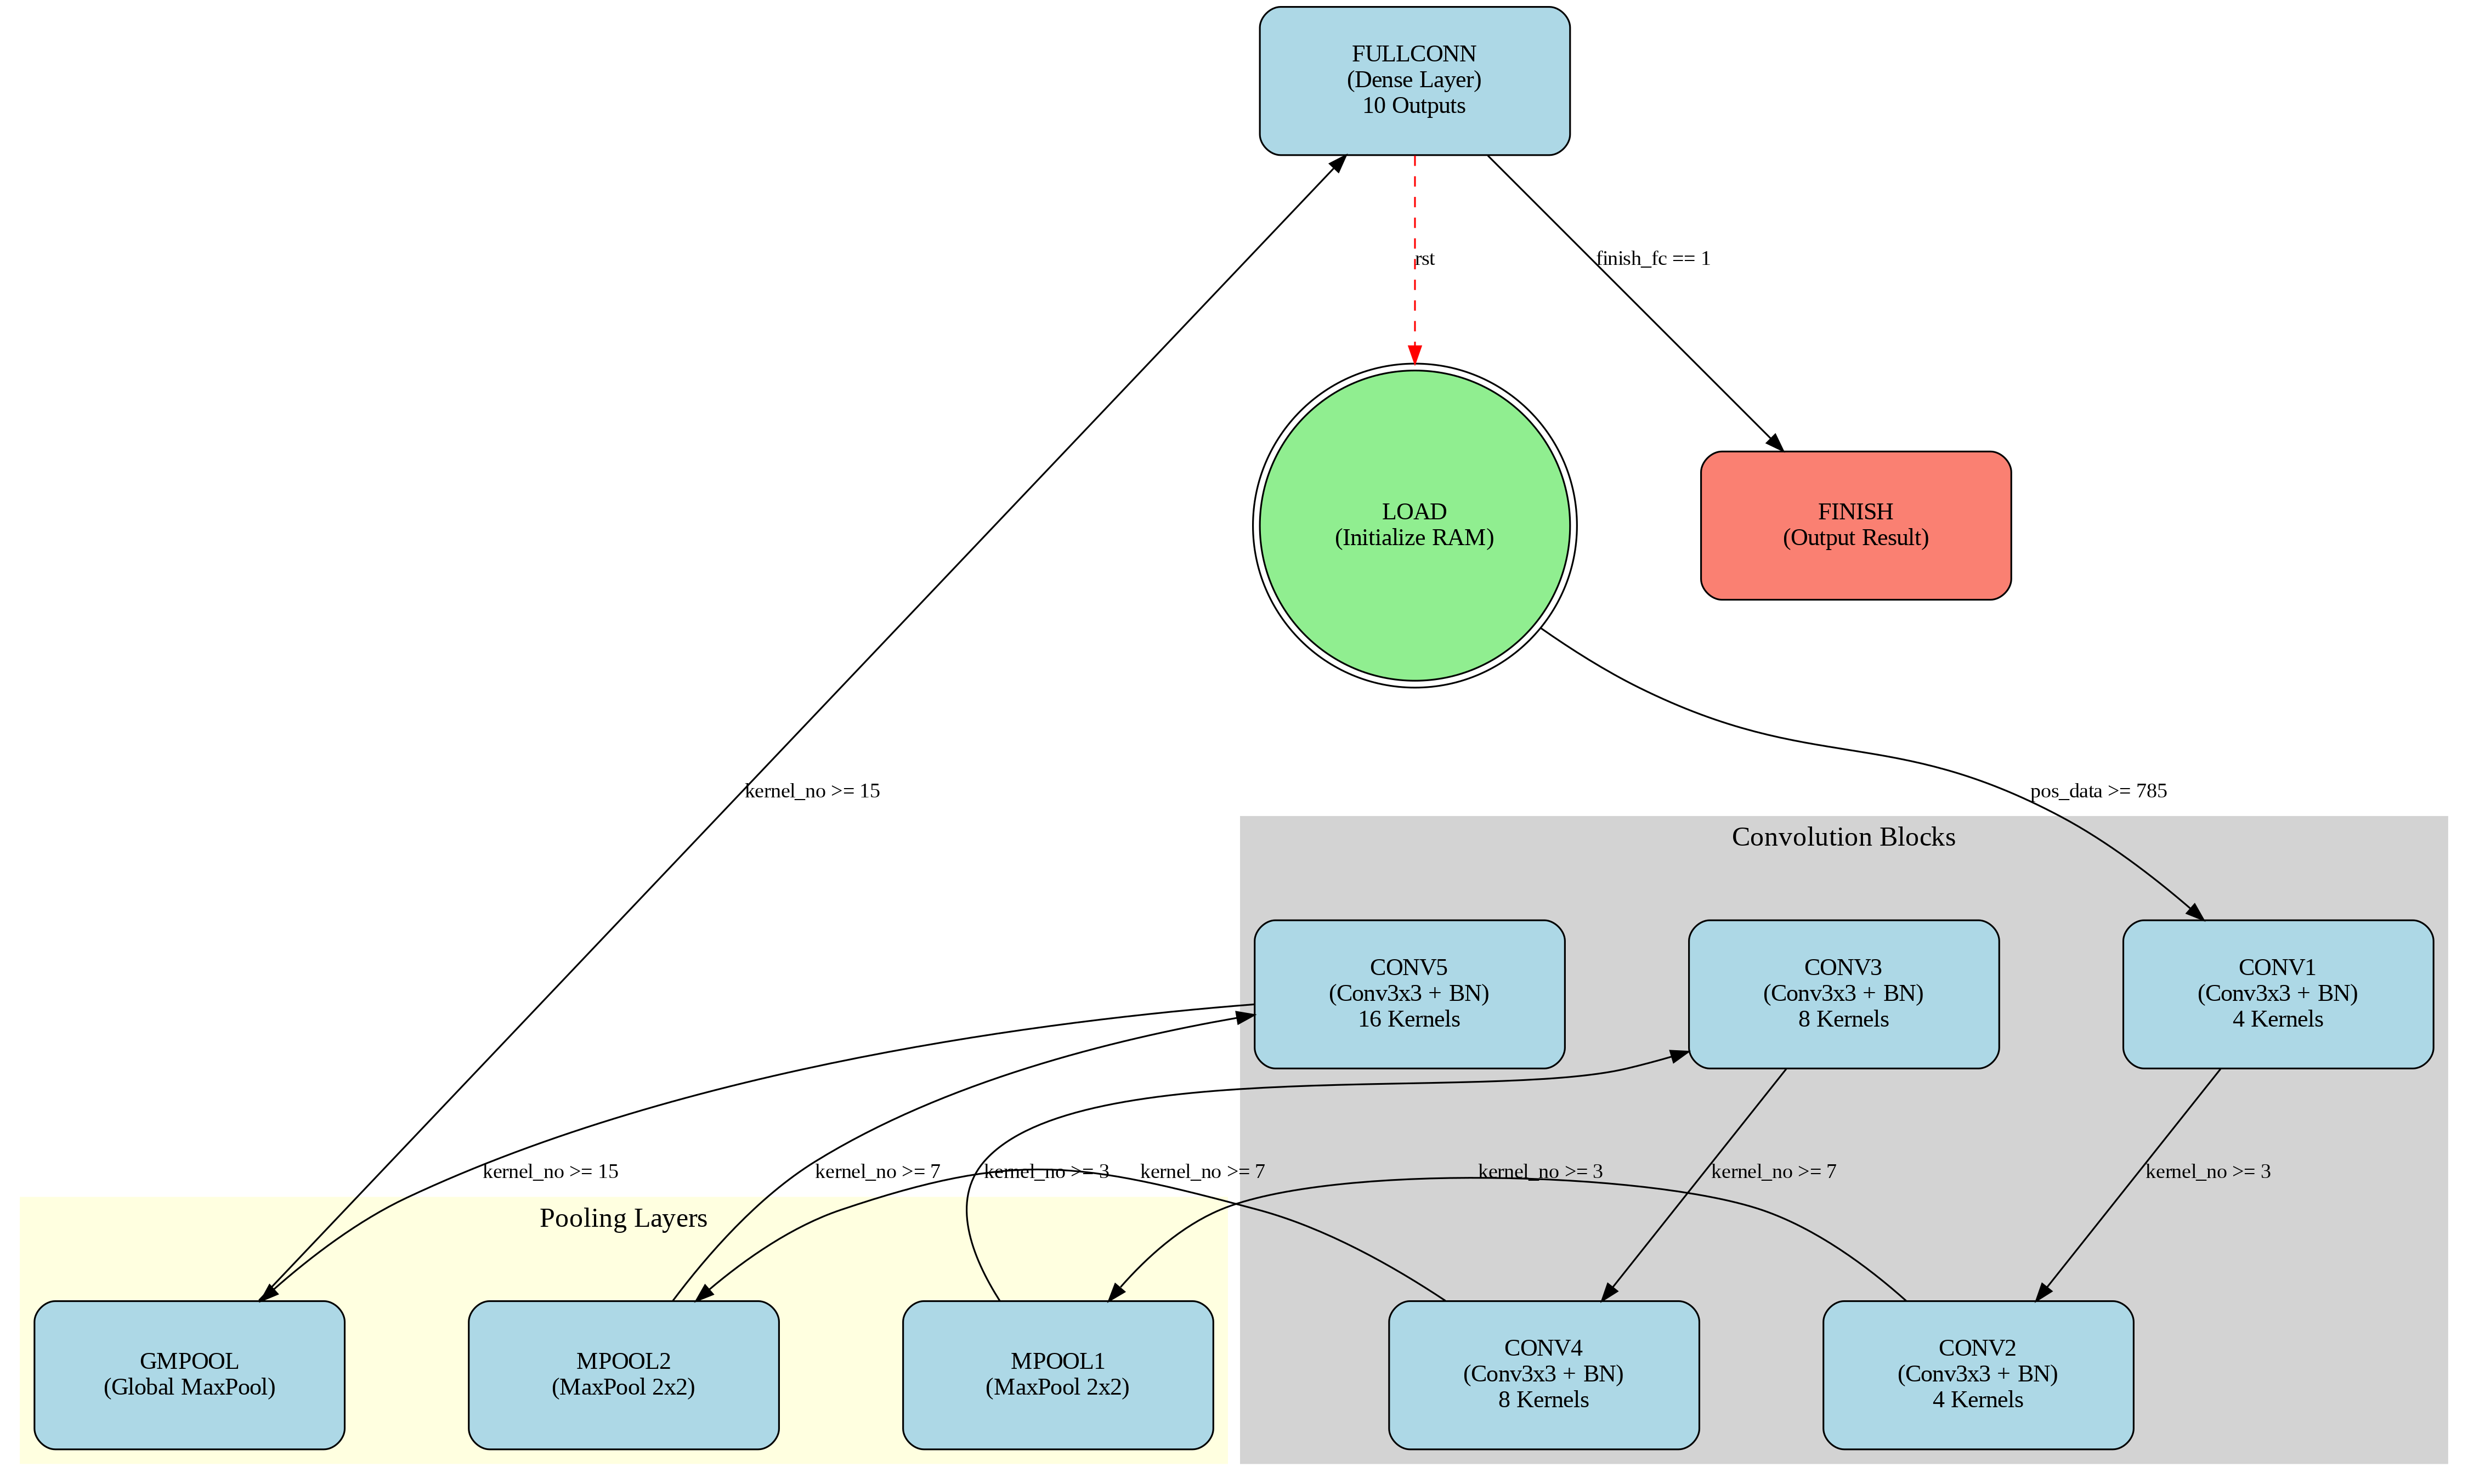
\includegraphics[width=0.9\linewidth]{Images/fsm.png}
    \caption{Sơ đồ trạng thái của khối điều khiển}
    \label{fig:enter-label}
\end{figure}
Ở các trạng thái khác nhau sẽ có tín hiệu điều khiển cho datapath khác nhau.

\subsubsection{Giai đoạn LOAD}
Ở giai đoạn này sẽ xuất các tín hiệu điều khiển để lưu ảnh mới 8-bit qua khối chuẩn hóa chuyển thành kiểu dữ liệu Q4.8 và lưu vào Bsram.
\begin{figure}[H]
    \centering
    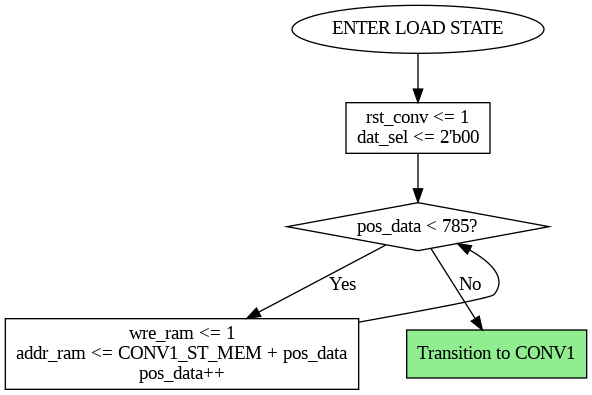
\includegraphics[width=0.75\linewidth]{Images/loadflow.png}
    \caption{Flow chart ở giai đoạn LOAD}
    \label{fig:enter-label}
\end{figure}

Kết thúc giai đoạn này ta sẽ có được 784 pixel dữ liệu hình ảnh đã được chuẩn hóa lưu ở trong Ram.

\subsubsection{Giai đoạn CONV1}
Ở giai đoạn ta cần điều khiển địa chỉ của ROM chứa trọng số của lớp Conv và BatchNormalize theo từng Kernel. Ngoài ra còn phải tính toán địa chỉ điểm ảnh của ảnh vừa được load vào trong Ram. Ảnh được load vào trong Ram là ảnh đã được làm phẳng do đó ta cần 2 thành ghi là \textit{x\_temp\_pos} và \textit{y\_temp\_pos} để thực hiện quá trình quét ảnh 2D của lớp Conv
\begin{figure}[H]
    \centering
    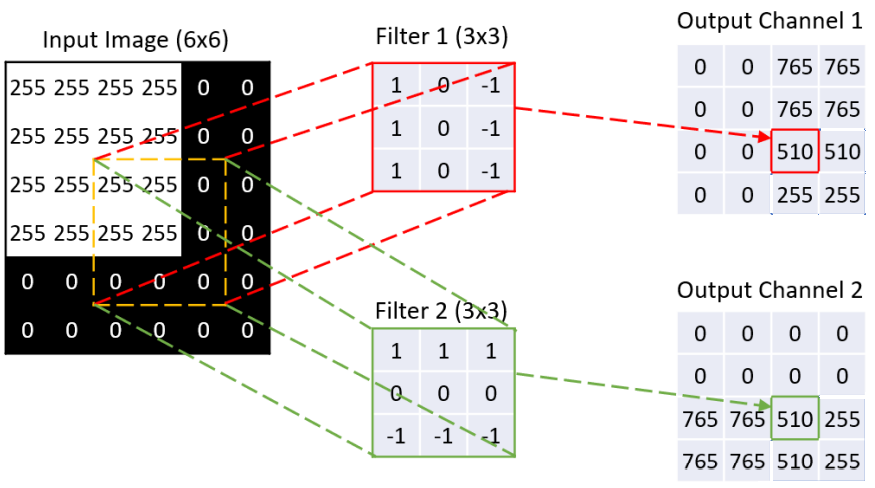
\includegraphics[width=0.75\linewidth]{Images/ohlc_filter.png}
    \caption{Quá trình quét ảnh 2D}
    \label{fig:filter}
\end{figure}
Ngoài 2 thanh ghi lưu tọa độ của điểm ảnh ta cần thêm 2 thanh ghi để lưu tọa độ 8 điểm ảnh lân cận. Vì như hình \ref{fig:filter} tất cả các Kernel (Filter) ta sử dụng trong mô hình này đều là 3x3 mỗi lần trượt của Filter sẽ lấy 9 giá trị điểm ảnh nhân tích chập với trọng số để tạo ra được điểm ảnh mới ở ngõ ra. \\
Và theo như mô hình ta chọn lúc đầu kích thước ảnh sau khi qua lớp Conv sẽ giữ nguyên (VD: 28x28) nhưng vì Kernel có size là 3x3 theo thực tế kích thước ảnh ngõ ra sẽ giảm 2 pixel (VD: 26x26). Vì thế ta sử dụng kỹ thuật Padding là các viền ngoài của ảnh ngõ vào sẽ cho bằng 0. Và theo như giải thuật trên ta sẽ thiết kế sao cho dựa vào 4 giá trị tọa độ điểm ảnh để phát hiện ra trường hợp điểm ảnh Padding.
\begin{figure}[H]
    \centering
    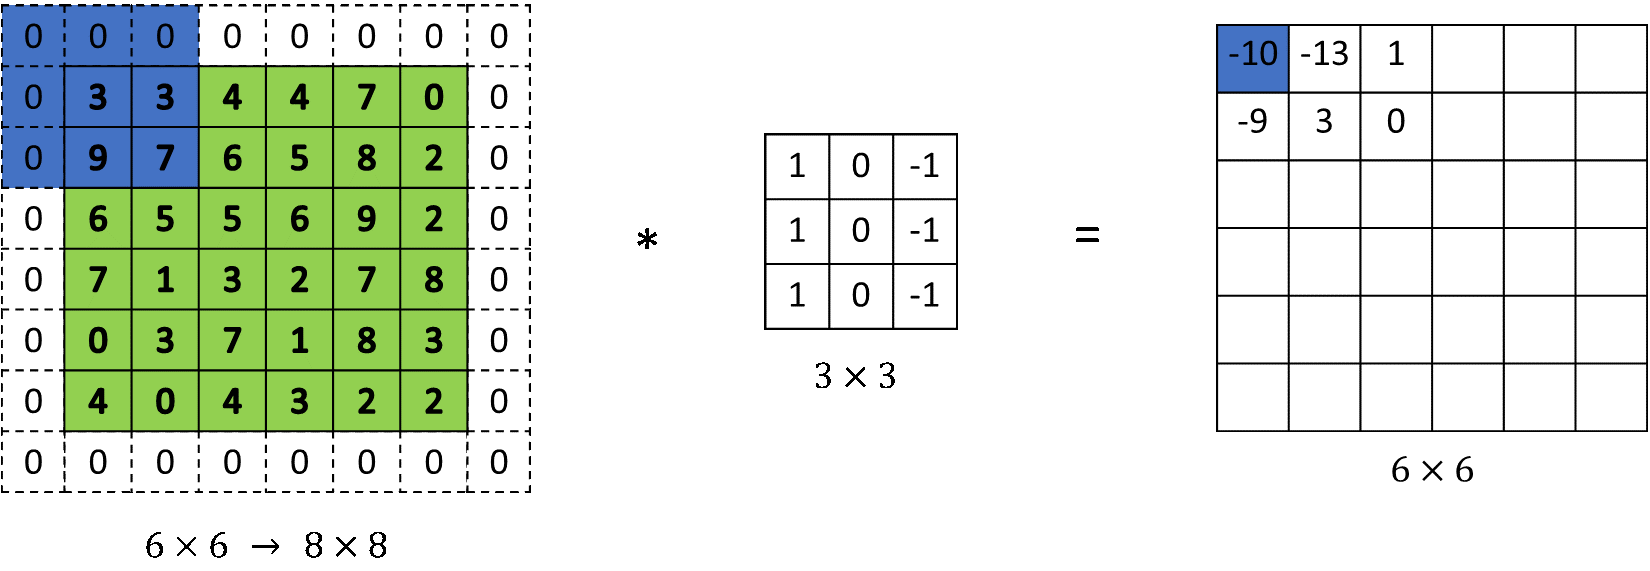
\includegraphics[width=0.9\linewidth]{Images/R.png}
    \caption{Padding cho lớp convolution}
    \label{fig:enter-label}
\end{figure}

Từ các ý trên ta có được các tín hiệu điều khiển như sau:


\begin{figure}[H]
    \centering
    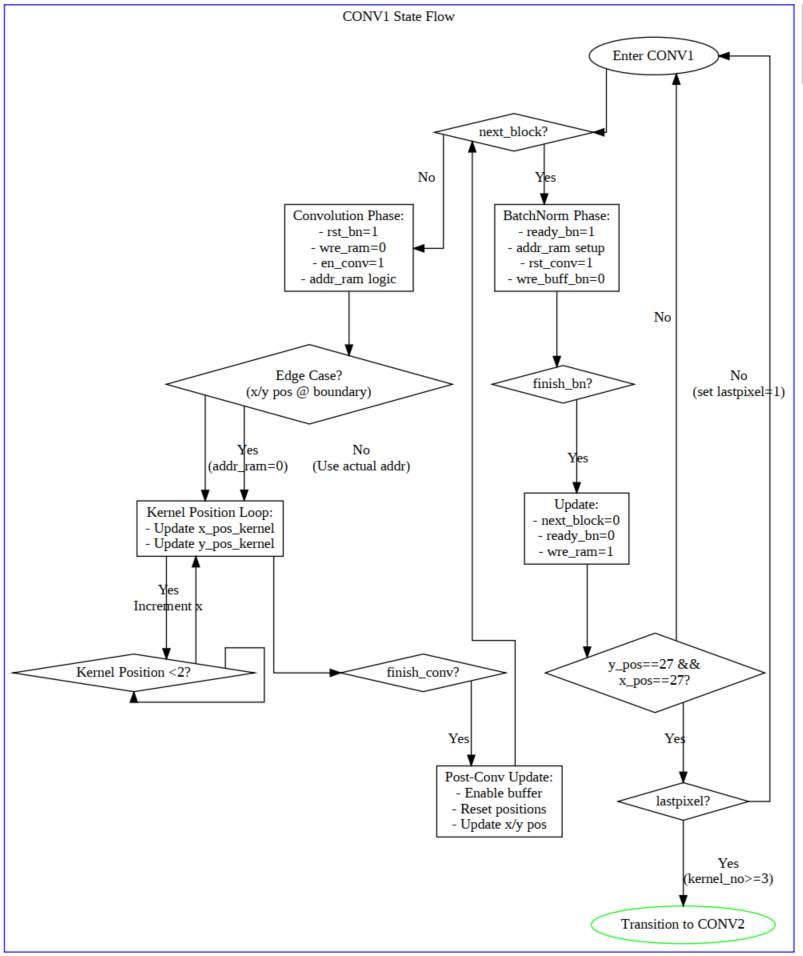
\includegraphics[width=0.75\linewidth]{Images/conv1flow.png}
    \caption{Flowchart CONV1}
    \label{fig:enter-label}
\end{figure}

Kết thúc giai đoạn CONV1 ta sẽ có được 4 kênh ảnh 28x28 mới lưu ở trong Ram và tiếp tục đến giai đoạn CONV2

\subsubsection{Giai đoạn CONV2}
Ở giai đoạn CONV2 sẽ tương tự giai đoạn đầu tiên, tuy nhiên số lượng ảnh kênh ngõ vào đã tăng lên thành 4 kênh. Như vậy ở mỗi Kernel ứng với mỗi kênh ảnh sẽ có mỗi Filter khác nhau (Window). 
\begin{figure}[H]
    \centering
    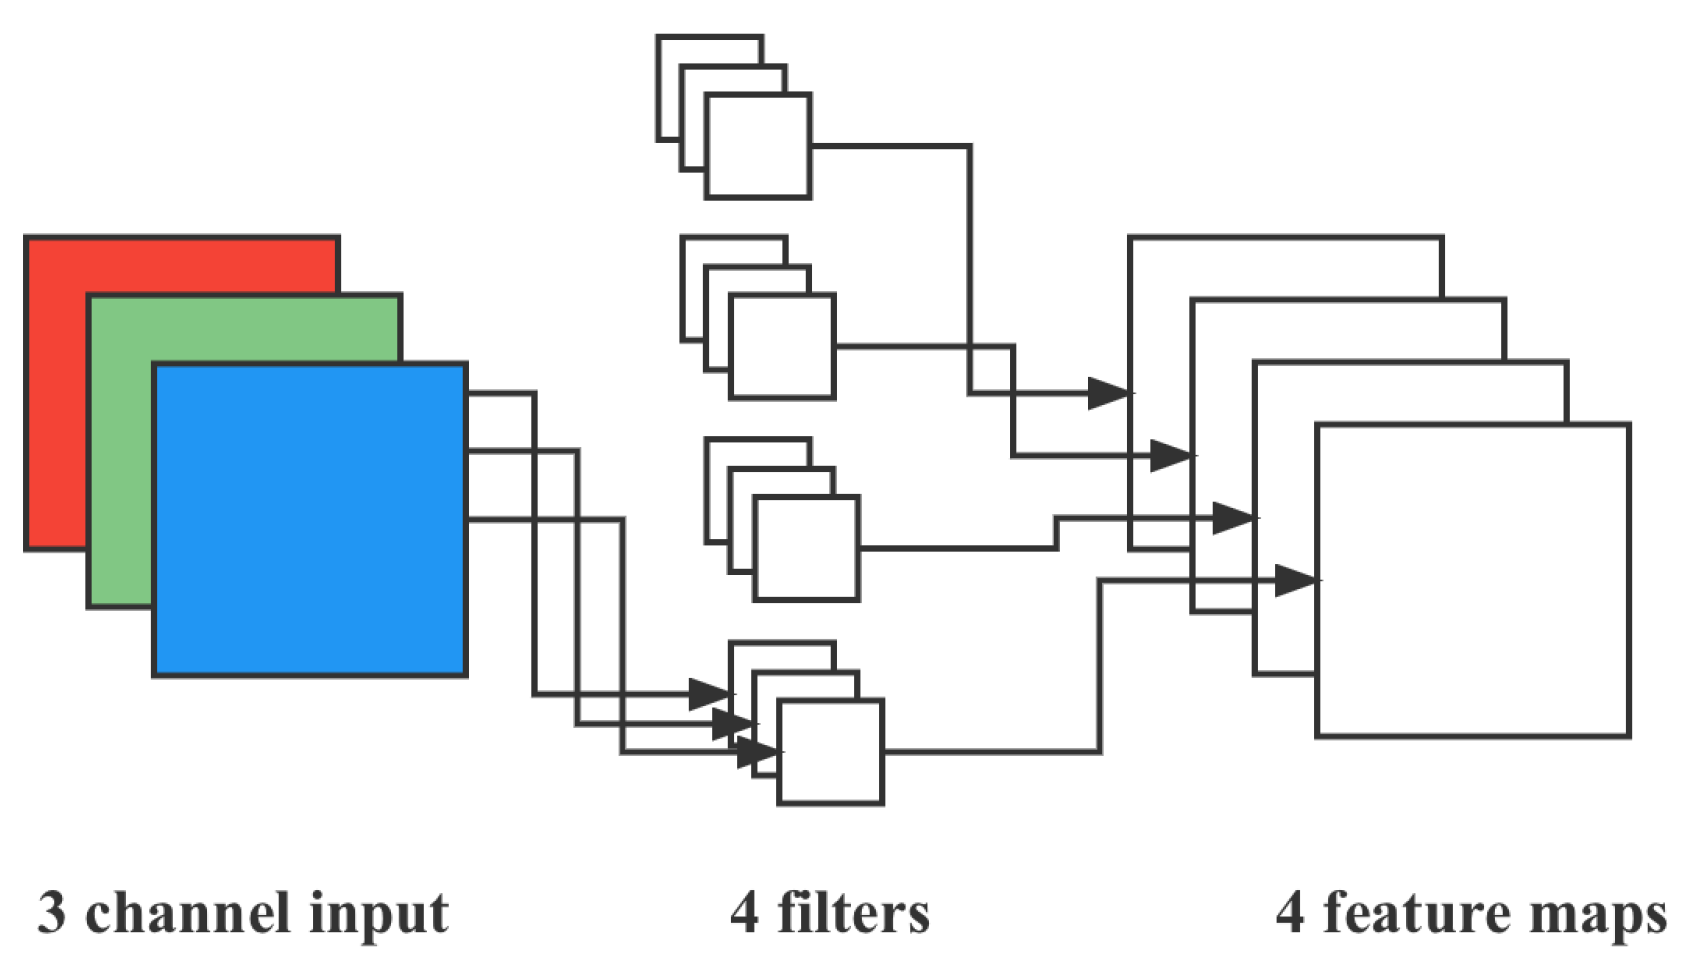
\includegraphics[width=0.75\linewidth]{Images/drones-06-00152-g010.png}
    \caption{Tích chập với ngõ vào nhiều kênh}
    \label{fig:enter-label}
\end{figure}
Vì thế tại mỗi điểm ảnh của mỗi kênh ngõ ra CONV2 sẽ là tổng tích chập của 4 kênh ảnh ngõ vào và 4 Window nên trong sơ đồ thiết kế phần cứng ta mới có thêm thanh ghi đệm Bnorm Reg trước khối BatchNormalize và bộ cộng để thực hiện điều này. Lúc này ở giai đoạn CONV2 ta cần phối hợp điều khiển thêm 2 tín hiệu là \textit{rst\_buff\_bn} và \textit{wre\_buff\_bn} để reset và cho phép ghi thanh ghi đệm này.
\begin{figure}[H]
    \centering
    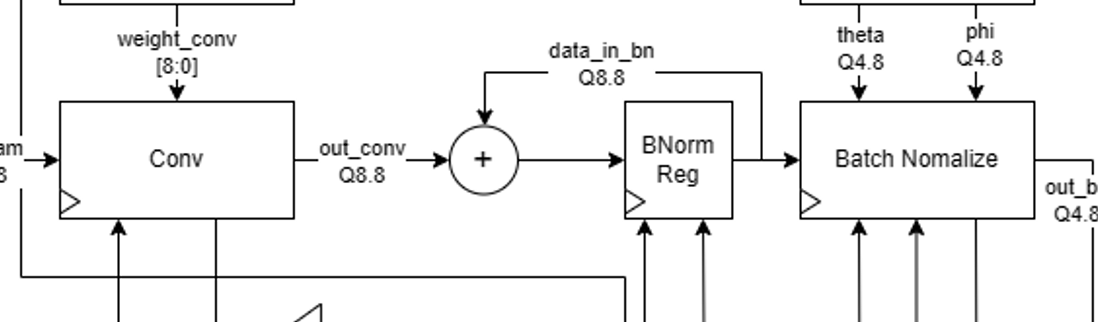
\includegraphics[width=0.75\linewidth]{Images/buffbn.png}
    \caption{Thanh ghi đệm Bnorm}
    \label{fig:enter-label}
\end{figure}
Ta lập được sơ đồ điều khiển các tín hiệu như sau:

\begin{figure}[H]
    \centering
    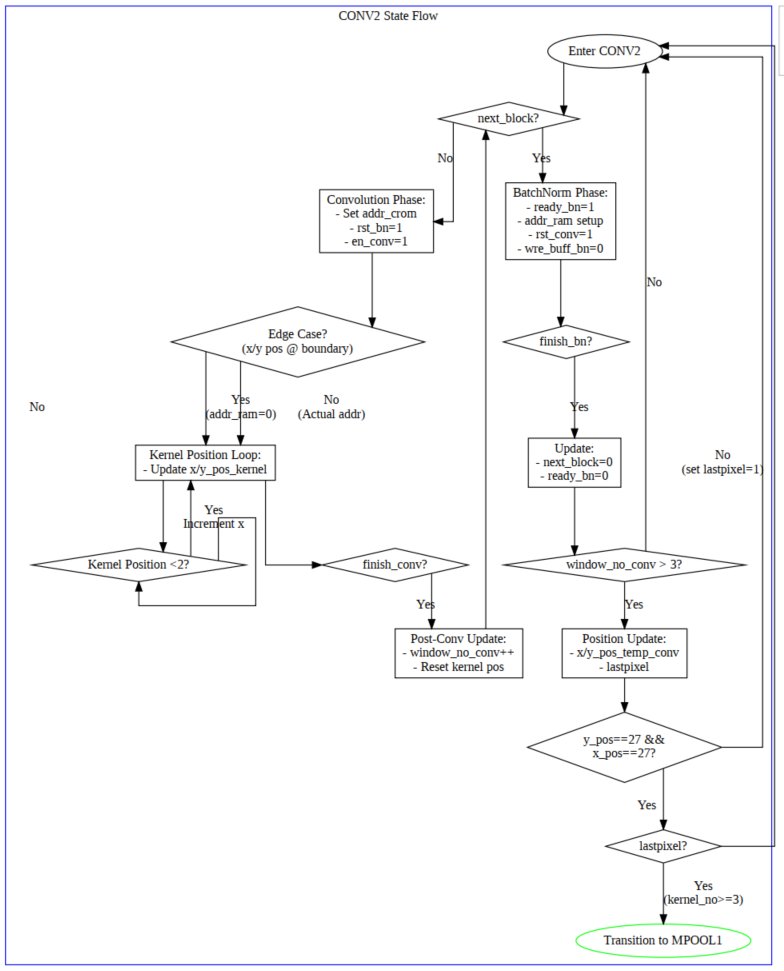
\includegraphics[width=0.75\linewidth]{Images/conv2flow.png}
    \caption{Flowchart CONV2}
    \label{fig:enter-label}
\end{figure}

Kết thúc giai đoạn CONV2 ta sẽ có được 4 kênh ảnh 28x28 mới và tiếp tục đến giai đoạn MAXPOOL1

\subsubsection{Giai đoạn MAXPOOL1}
Với giai đoạn max pooling 2D này ta sẽ so sánh 4 giá trị điểm ảnh trong vùng không gian 2x2 trên ảnh 2 chiều và chọn ra điểm ảnh có giá trị lớn nhất. Với kỹ thuật này sẽ giảm nửa chiều dữ liệu ngõ vào cho lớp sau.

\begin{figure}[H]
    \centering
    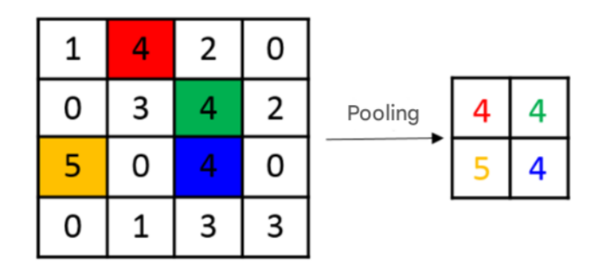
\includegraphics[width=0.75\linewidth]{Images/pooling.png}
    \caption{Maxpooling 2D}
    \label{fig:enter-label}
\end{figure}

Ta lập được sơ đồ điều khiển các tín hiệu cho giai đoạn max pooling như sau:

\begin{figure}[H]
    \centering
    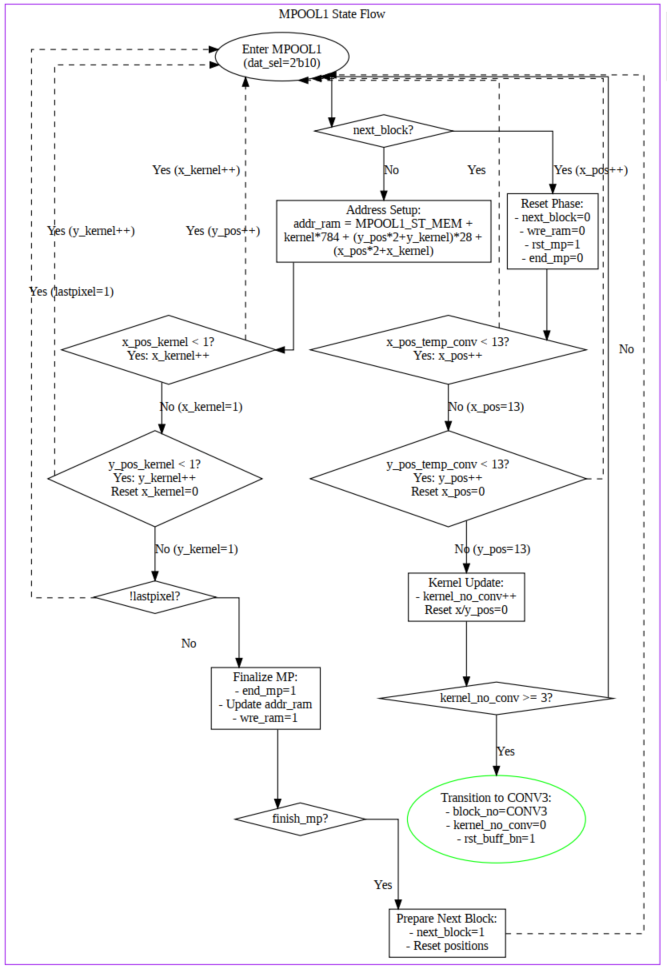
\includegraphics[width=0.75\linewidth]{Images/mpoolflow.png}
    \caption{Flowchart MAXPOOL1}
    \label{fig:enter-label}
\end{figure}
Kết thúc giai đoạn MAXPOOL1 ta sẽ có được 4 kênh ảnh 14x14 mới lưu ở trong Ram và tiếp tục đến giai đoạn CONV3

\subsubsection{Giai đoạn CONV3}
Giai đoạn này gần giống với CONV2 với số Kernel là 8 và số Window là 4. Và dữ liệu hình ảnh lúc này là 14x14 nên ta cần giảm số vòng lặp và thông số vị trí vùng Padding.\\
Kết thúc giai đoạn CONV3 ta sẽ có được 8 kênh ảnh 14x14 mới lưu ở trong Ram và tiếp tục đến giai đoạn CONV4.

\subsubsection{Giai đoạn CONV4}
Giai đoạn này giống với giai đoạn CONV3 với số lượng Window lúc này là 8.\\
Kết thúc giai đoạn CONV4 ta sẽ có được 8 kênh ảnh 14x14 mới lưu ở trong Ram và tiếp tục đến giai đoạn MAXPOOL2.

\subsubsection{Giai đoạn MAXPOOL2}
Tương tự giai đoạn MAXPOOL1 lúc này ta sẽ giảm một nửa dữ liệu. Lúc này dữ liệu ảnh cho giai CONV5 sau là 8 kênh anh 7x7.

\subsubsection{Giai đoạn CONV5}
Giai đoạn này giống với các giai đoạn CONV trên với số lượng Kernel là 16, Window là 8 tương ứng với 8 kênh ảnh 7x7 ở ngõ vào.\\
Kết thúc giai đoạn CONV5 ta sẽ có được 16 kênh ảnh 7x7 mới lưu ở trong Ram và tiếp tục đến giai đoạn GMPOOL.

\subsubsection{Giai đoạn GMPOOL}
Như đã nói ở các phần trước nhằm để giảm số lượng trọng số và tính toán ở lớp Fully Connect ta sử dụng kỹ thuật giảm chiều dữ liệu này với 16 kênh ảnh 7x7 từ giai đoạn trước đó.
\begin{figure}[H]
    \centering
    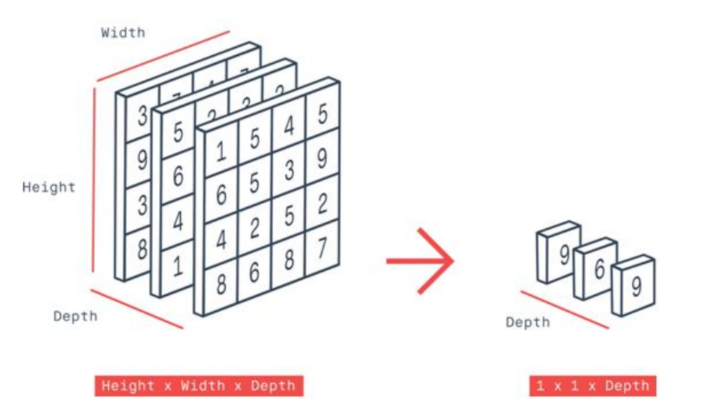
\includegraphics[width=0.75\linewidth]{Images/gmpool2.png}
    \caption{Kỹ thuật global max pool}
    \label{fig:enter-label}
\end{figure}
Điều khiển các tín hiệu tướng tự Max Pooling ta có được flow chart sau:
\begin{figure}[H]
    \centering
    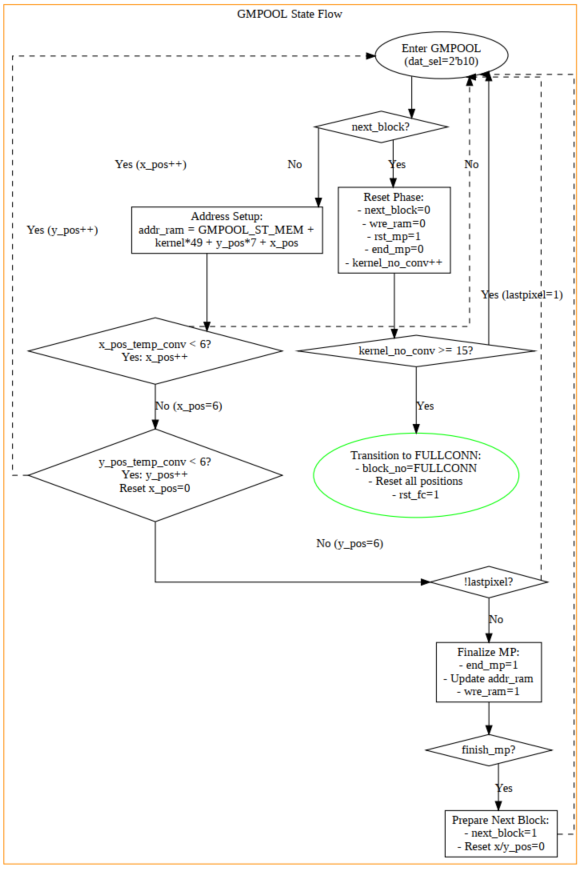
\includegraphics[width=0.75\linewidth]{Images/gmpoolflow.png}
    \caption{Flowchart GlobalMaxPooL}
    \label{fig:enter-label}
\end{figure}
Kết thúc giai đoạn GMPOOL ta sẽ có được 16 kênh ảnh 1x1 mới lưu ở trong Ram và tiếp tục đến giai đoạn FULLYCONN.

\subsubsection{Giai đoạn FULLYCONN}
Với ngõ vào là 16 kênh tương ứng ta có 16 Window, ngõ ra 10 kênh ứng với 10 Kernel. Sử dụng các thanh ghi để làm bộ đếm để lấy đúng dữ liệu trọng số ứng với Kernel và Window từ ROM và đưa váo khối FullyConnect.

\begin{figure}[H]
    \centering
    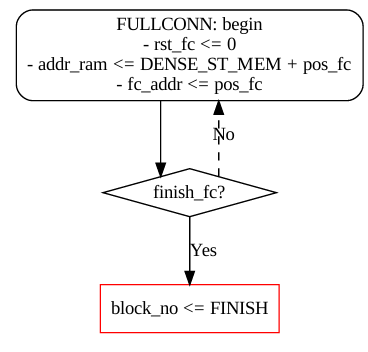
\includegraphics[width=0.5\linewidth]{Images/fcflow.png}
    \caption{Flowchart FULLYCONN}
    \label{fig:enter-label}
\end{figure}

Kết thúc quá trình load dữ liệu khối fully connect sẽ tự tính toàn và so sánh để đưa ra kết quả dự đoán số viết tay. Máy trạng thái sẽ chuyển qua trạng thái FINISH, kich hoạt cờ finish, để thực hiện chu trình dự đoán tiếp theo chỉ cần đưa tín hiệu reset cho máy trạng thái. 

\subsection{CNN Top}
\subsubsection{Thiết kế khối CNN Top}
Dựa vào sơ đồ thiết kế phần cứng (Hình \ref{fig:tkpc}) ta kết nối khối điều khiển và datapath với nhau để hoàn chỉnh module nhận diện số viết tay.
\begin{table}[H]
\centering
\caption{CNN Module Signal Definitions}
\label{tab:cnn_signals}
\begin{tabular}{llll}
\toprule
\textbf{Signal Name} & \textbf{Direction} & \textbf{Width} & \textbf{Description} \\ 
\midrule
clk & Input & 1 & System clock \\
rst & Input & 1 & Active-high reset \\
en & Input & 1 & Module enable control \\
data\_in & Input & 8 & Input pixel data (unsigned byte) \\ 
pos\_data & Output & 10 & Position counter/address bus \\
finish & Output & 1 & Operation completion flag \\
cnn\_out & Output & 4 & Classification result (0-9) \\ 
\bottomrule
\end{tabular}
\end{table}

\subsubsection{Synthesize}
Sử dụng tool Gowin để synthesis ta có báo cáo sử dụng tài nguyên như bảng \ref{tab:resource_usage_summary}.
\begin{table}[H]
\centering
\caption{Resource Usage Summary}
\label{tab:resource_usage_summary}
\begin{tabular}{ll}
\toprule
\textbf{Resource} & \textbf{Usage} \\
\midrule
I/O Port & 26 \\
I/O Buf & 25 \\
\quad $\bullet$ IBUF & 10 \\
\quad $\bullet$ OBUF & 15 \\
Register & 410 \\
\quad $\bullet$ DFF & 16 \\
\quad $\bullet$ DFFE & 34 \\
\quad $\bullet$ DFFRE & 1 \\
\quad $\bullet$ DFFPE & 103 \\
\quad $\bullet$ DFFC & 6 \\
\quad $\bullet$ DFFCE & 250 \\
LUT & 1353 \\
\quad $\bullet$ LUT2 & 289 \\
\quad $\bullet$ LUT3 & 352 \\
\quad $\bullet$ LUT4 & 712 \\
ALU & 1039 \\
\quad $\bullet$ ALU & 1039 \\
SSRAM & 3 \\
\quad $\bullet$ RAM16S4 & 3 \\
INV & 17 \\
\quad $\bullet$ INV & 17 \\
DSP & - \\
\quad $\bullet$ MULT18X18 & 10 \\
\quad $\bullet$ MULTADDALU18X18 & 5 \\
BSRAM & 15 \\
\quad $\bullet$ SP & 12 \\
\quad $\bullet$ pROM & 2 \\
\quad $\bullet$ pROMX9 & 1 \\
\bottomrule
\end{tabular}
\end{table}

Ta thấy thiết kế sử dụng rất ít tài nguyên với 2427 LUT, 410 thanh ghi flipflop và 15x16kbit bộ nhớ Ram.
\begin{table}[H]
\centering
\caption{Resource Utilization Summary}
\label{tab:resource_utilization_summary}
\begin{tabular}{l r@{\hspace{1em}}l S[table-format=2.1]}
\toprule
\multirow{2}{*}{\textbf{Resource}} & 
\multicolumn{2}{c}{\textbf{Used/Total}} & 
\multirow{2}{*}{\textbf{Utilization}} \\
& \multicolumn{2}{c}{(units)} & \\
\midrule
Logic & 2427 (1370 LUT, 1039 ALU, 3 RAM16) & / 8640 & 29.0\% \\
Register & 410 & / 6693 & 7.0\% \\
\quad $\bullet$ Register as Latch & 0 & / 6693 & 0.0\% \\
\quad $\bullet$ Register as FF & 410 & / 6693 & 7.0\% \\
BSRAM & 15 & / 26 & 58.0\% \\
\bottomrule
\end{tabular}
\end{table}

\subsubsection{Verification Plan}
\begin{table}[H]
\centering
\caption{CNN Module Verification Plan}
\begin{tabular}{>{\bfseries}p{2.5cm}p{4cm}p{4cm}p{3cm}}
\toprule
\textbf{Test Category} & \textbf{Test Case} & \textbf{Verification Method} & \textbf{Expected Result} \\
\midrule

Reset Verification & Power-on reset & Assert reset for 10 cycles & All states reset to LOAD, pos\_data=0, finish=0 \\
\hline
Convolution Layers & CONV1 edge pixels & Input boundary coordinates (x=0, y=0) & Zero-padded address (addr\_ram=0) selected \\
\hline
BatchNorm Integration & Post-CONV1 processing & Monitor bn\_addr and wre\_buff\_bn & Correct BN parameters applied to conv output \\
\hline
Max Pooling & MPOOL1 downsampling & Input 4x4 pattern with max=255 & Output 2x2 max values at correct addresses \\
\hline
State Transitions & CONV1→CONV2 transition & Trigger finish\_bn signal & block\_no increments to CONV2 within 1 cycle \\
\hline
Memory Addressing & CONV3 weight fetching & Check addr\_crom during computation & Correct CROM offset (20 + kernel\_no*4 + window\_no) \\
\hline
Global Pooling & GMPOOL operation & Feed 7x7 input with single peak & Maximum value stored at DENSE\_ST\_MEM \\
\hline
Full Connection & Final classification & Load precomputed GMPOOL outputs & cnn\_out matches MNIST label (one-hot) \\
\hline
Error Recovery & Mid-process reset & Assert rst during CONV2 operation & Immediate return to LOAD state \\
\hline
MNIST Accuracy & 10k test images & Compare cnn\_out with labels & ≥98\% classification accuracy \\

\bottomrule
\end{tabular}
\end{table}
Từ kế hoạch kiểm thử trên ta sẽ kiểm tra thiết kế ở phần sau.